% Base Template: https://www.overleaf.com/latex/templates/th-koln-2018-template-for-web-science-master-thesis/hcbvkhmvddbz
%Dokumentklasse
\documentclass[a4paper,12pt,makeidx,twoside,openright,numbers=noenddot]{scrreprt}
\usepackage[left=3cm, right=2cm, bottom=2.5cm, top=3cm]{geometry}		% Formatierung der Seitenränder
%\usepackage[onehalfspacing]{setspace}							        % verwendet für größeren Zeilenabstand

% ============= Packages =============

% Dokumentinformationen
\usepackage[
	pdftitle={},
	pdfsubject={},
	pdfauthor={},
	pdfkeywords={},
	%Links nicht einrahmen
	hidelinks
]{hyperref}

\usepackage[utf8]{inputenc}
\usepackage[english]{babel}
\usepackage[T1]{fontenc}
\usepackage{units}
\usepackage{pdfpages}
\usepackage{listings}
\usepackage{svg}					% Zur Einbindung von scalable vector graphics
\usepackage{subcaption}				% Zum Einbinden von Untergrafiken
\usepackage[gen]{eurosym}			% Zur Verwendung des Eurozeichens
\usepackage{amssymb}
\usepackage{graphicx}
\graphicspath{{img/}}				
\usepackage{fancyhdr}				% Style Package für's Seitenlayout
\usepackage{color}					% anpassen von Farben
\usepackage{microtype} 				% schönerer Blocksatz!
\usepackage{calc}  					
\usepackage{enumitem}				% zb für align der description
\usepackage[font=small,labelfont=bf]{caption}
\usepackage[printonlyused]{acronym}	% für Abkürzungen
\usepackage{multicol}
\usepackage{booktabs}
\usepackage{textcomp}
\usepackage{listings}				% Einbindung von Code in LateX
\usepackage{setspace}
\usepackage{threeparttable} 		% für Fußnoten innerhalb einer Tabelle
\usepackage[export]{adjustbox}


% verschiedene Schriftarten
%\usepackage{times} 				% times font
%\usepackage{palatino}			 	% Palatino font
\usepackage{lmodern}				% Lmodern sans und serif
%\usepackage{libertine}				% Linux Libertine und Biolinum

%\usepackage{fontspec}				% Nutzen in Kombination mit LuaLaTeX, um Systemschriften einzubinden
%\setmainfont{Georgia}				% beispielsweise Georgia, aber auch jede andere Schrift, die auf dem PC vorhanden ist


% zusätzliche Schriftzeichen der American Mathematical Society
\usepackage{amsfonts}
\usepackage{amsmath}

\usepackage[numbers, comma]{natbib}		% Einstellung des Zitierstils
\bibliographystyle{lni_style}			% Angepasster Stil für deutsche Sprache

\setcounter{secnumdepth}{3}				% Nummerierungsebene anpassen -> 3 = subsubsection werden nummeriert
\setcounter{tocdepth}{1}   				% gliederungsebenen im Inhaltsverzeichnis -> erstmal nur zur übersicht was nicht vergessen werden darf

\definecolor{deepblue}{rgb}{0,0,0.5}
\definecolor{deepred}{rgb}{0.6,0,0}
\definecolor{deepgreen}{rgb}{0,0.5,0}


% ============= Kopf- und Fußzeile =============
\pagestyle{fancy}

%% Formatierung der Kopf- und Fußzeile
\fancyhead{}
\fancyhead[RO,LE]{\thepage}
\fancyhead[RE]{\leftmark}
\fancyhead[LO]{\rightmark}
%%
\fancyfoot{}

\renewcommand{\headrulewidth}{0.4pt}		% Bei zweiseitigem Dokument ausschließlich Linie in Kopfzeile
\renewcommand{\chaptermark}[1]{\markboth{\thechapter\ #1}{}}
\renewcommand{\sectionmark}[1]{\markright{\thesection\ #1}}

% ============= Package Einstellungen & Sonstiges ============= 
% Besondere Trennungen
\hyphenation{Um-ge-bungs-tem-pe-ra-tur Um-ge-bungs-tem-pe-ra-tur-en Rauch-gas-tem-pe-ra-tur Aus-tritts-tem-pe-ra-tur}

% Einstellung wie Code innerhalb der Arbeit gesetzt werden soll:
\lstdefinestyle{Style}{
	columns=flexible,
	basicstyle=\ttfamily}
\lstset{ 
	backgroundcolor=\color{white},   % choose the background color; you must add \usepackage{color} or \usepackage{xcolor}; should come as last argument
	basicstyle=\footnotesize,        % the size of the fonts that are used for the code
	breakatwhitespace=false,         % sets if automatic breaks should only happen at whitespace
	breaklines=true,                 % sets automatic line breaking
	captionpos=none,                 % sets the caption-position to bottom
	commentstyle=\color{deepblue},   % comment style
	deletekeywords={...},            % if you want to delete keywords from the given language
	escapeinside={\%*}{*)},          % if you want to add LaTeX within your code
	extendedchars=true,              % lets you use non-ASCII characters; for 8-bits encodings only, does not work with UTF-8
	firstnumber=1,               	 % start line enumeration with line 1000
	frame=single,	                 % adds a frame around the code
	keepspaces=true,                 % keeps spaces in text, useful for keeping indentation of code (possibly needs columns=flexible)
	keywordstyle=\color{blue},       % keyword style
	language=Python,                 % the language of the code
	morekeywords={*,...},            % if you want to add more keywords to the set
	numbers=left,                    % where to put the line-numbers; possible values are (none, left, right)
	numbersep=5pt,                   % how far the line-numbers are from the code
	emphstyle=\color{deepred},
	%numberstyle=\tiny\color{mygray}, % the style that is used for the line-numbers
	rulecolor=\color{black},         % if not set, the frame-color may be changed on line-breaks within not-black text (e.g. comments (green here))
	showspaces=false,                % show spaces everywhere adding particular underscores; it overrides 'showstringspaces'
	showstringspaces=false,          % underline spaces within strings only
	showtabs=false,                  % show tabs within strings adding particular underscores
	stepnumber=2,                    % the step between two line-numbers. If it's 1, each line will be numbered
	stringstyle=\color{deepgreen},     % string literal style
	tabsize=2,	                   	 % sets default tabsize to 2 spaces
	title=\lstname                   % show the filename of files included with \lstinputlisting; also try caption instead of title
}

% nicht einrücken nach Absatz
\setlength{\parindent}{0pt}
\usepackage{parskip}		 			% verhindert einrücken und setzt einen kleinen Absatz

\renewcommand{\arraystretch}{1.2}		% Abstand innerhalb der Tabellen einstellen
\usepackage[utf8]{inputenc}

\newcommand*{\mytitle}{Self-sovereign Identity: \\Development of an Implementation-based Evaluation Framework for Verifiable Credential SDKs} % Titel
\newcommand*{\myinstitute}{Brandenburg University of Applied Sciences} % Institut
\newcommand*{\myfaculty}{Department of Economics} % Weitere Hinweise
\newcommand*{\myauthor}{Philipp Bolte} % Autoren
\newcommand*{\myreporttype}{Master's Thesis} % Typ
\newcommand*{\mydate}{\today} % Datum


% ============= Dokumentbeginn =============

\begin{document}
	
% Seiten ohne Kopf- und Fußzeile sowie Seitenzahl
\pagestyle{empty}


\begin{center}
\begin{tabular}{p{\textwidth}}

\begin{center}

\includegraphics[scale=0.25, left]{img/0_logo.eps}
\end{center}

\\\\\\\

\begin{center}
\LARGE{\textbf{
\mytitle\\[1cm]
}}
\end{center}

\\

\begin{center}
\large{\myinstitute\\
\myfaculty\\}
\end{center}

\\\\\\\\\\\\

\begin{center}
\textbf{\Large{\myreporttype}}
\end{center}

\\\\

\begin{center}
submitted by
\end{center}

\begin{center}
\large{\textbf{\myauthor}} \\
% \small{geboren am 01.01.0001 in Entenhausen}
\end{center}

\begin{center}
\large{\mydate}
\end{center}

\\\\\\\\\\

\begin{center}
\begin{tabular}{lll}
\textbf{First supervisor:} & & Prof. Dr. rer. nat. Vera G. Meister\\
\textbf{Second supervisor:} & & Jonas Jetschni, M.Sc.\\
\end{tabular}
\end{center}

\end{tabular}
\end{center}	% Einbinden der Titelseite
\newpage 					% Um Seite nach der Titelseite einzubinden -> bei eigener Titelseite und nicht der Latex-Version erforderlich
\thispagestyle{empty}
\quad 
\newpage
\pagenumbering{Roman}
 
\cleardoubleoddpage


\chapter*{Statutory Declaration}
I hereby attest that I have written this thesis independently without any outside help and that I have used only the sources cited. \\~\\
Brandenburg, \today\\[.6cm]
Philipp Bolte\\
\rule[0.5em]{20em}{0.5pt}

\chapter*{Abstract}

In an increasingly globalized and digitized world, the functioning of societies depends on digital identities. These are commonly based on centralized or federated technologies controlled by private organizations. Self-sovereign identity offers a new approach to digital identities, giving complete control back to users and breaking dependencies on middlemen. Previous literature on this has mostly focused on foundational work and less on practical developer-oriented topics. This thesis tries to close this gap by providing an overview of existing solutions and by presenting a new evaluation framework for such solutions based on a reference implementation. The goal is to provide a baseline to support developers in integrating Self-sovereign identity into their projects.

\textit{In einer zunehmend globalisierten und digitalisierten Welt ist das Funktionieren von Gesellschaften von digitalen Identitäten abhängig. Diese basieren häufig auf zentralisierten oder föderierten Technologien kontrolliert durch privaten Organisationen. Self-sovereign Identity bietet dabei einen neuen Ansatz für digitale Identitäten, in dem den Nutzern die komplette Kontroller zurückgegeben wird und die Abhängigkeiten zu oft unsicheren Mittelsmännern aufgelöst wird. Bisherige Literatur hatte sich dazu vorwiegend auf Grundlagenarbeit und weniger auf praxisrelevante, entwicklerorientierte Themen konzentriert. Diese Lücke wird in dieser Arbeit versucht zu schließen, in dem zum einen eine Übersicht über bestehende Lösungen angefertigt wird und zum anderen ein neues Bewertungsrahmenwerk für solche Lösungen auf Basis einer Referenzimplementierung vorgestellt wird. So sollen erste Grundlagen geschaffen werden, um Entwickler bei der Integration von Self-sovereign Identity in ihre Projekte zu unterstützen.}



\tableofcontents			%Inhaltsverzeichnis
\listoffigures				%Verzeichnis aller Bilder
\listoftables				%Verzeichnis aller Tabellen
\chapter*{List of Abbreviations}
    \begin{acronym}[SDK]
        \acro{DID}{Decentralized Identifier}
        \acro{sdk}[SDK]{Software Development Kit}
        \acroplural{sdk}[SDKs]{Software Development Kits}
        \acro{SSI}{Self-sovereign Identity}
        \acro{vc}[VC]{Verifiable Credential}
        \acroplural{vc}[VCs]{Verifiable Credentials}
        \acro{VP}{Verifiable Presentation}
        \acro{ca}[CA]{Certificate Authority}
        \acroplural{ca}[CAs]{Certificate Authorities}
    \end{acronym}

\pagestyle{fancy}

\chapter{Introduction}
\pagenumbering{arabic}
	The Internet has become a cornerstone of coexistence in today's world. With over 4.66 billion Internet users worldwide \cite{johnson_internet_2021}, it determines how we communicate, think, inform ourselves, and interact with one another.	As a result, huge networks of people are being created in which different cultures are coming closer together and knowledge is being shared like never before.
	A central enabler for the functioning of such interactions are digital identities, which are gaining an increasingly important role \cite{liu_blockchain-based_2020}.
	
	Over the course of our lives, we collect a large amount of digital identities from a wide variety of services, including Facebook, Twitter, WhatsApp, GitHub, LinkedIn, and many more. Because of the way we manage digital identities in the current era, users mostly own separate identities for each service or go through centralized, federated identity providers like Google or Facebook. As a result of these key developments, silos of identity data emerged, which are problematic concerning efficiency, security, and privacy. Several historical data leaks and hacks in which sensitive user data was made public show that these approaches are not suitable for managing sensitive user data. \cite{swinhoe_15_2021}. \cite{ehrlich_self-sovereign_2021}
	
	In contrast, the \ac{SSI} paradigm takes a new approach by giving back users control of their digital identities through various novel approaches. This thesis explores this new approach from a developer's point of view. In the next sections, the objectives, related work and the research approach will be discussed.
	
	\section{Objectives} % might be the wrong word; maybe objectives? Or "Motivation and Objectives"?
	
	For a successful realization of \acf{SSI} concepts, the existence of good solutions for developers is critical. This ensures that the barriers to a successful adoption of \ac{SSI} are kept to a minimum, simplifying and speeding up the entire process. A good toolset and developer experience is thus a key enabler for \ac{SSI}.
	
	With this in mind, an overview of the most important solutions\footnote{synonymous to SDKs, libraries, frameworks, and platforms} in the \ac{SSI} space will be established throughout the thesis. To scope the work accordingly, this thesis looks at the solutions in terms of how closely they can map the lifecycle of a \acf{VC}. It is intended to serve as an entry point for developers to get an overview of the capabilities of existing solutions and to give starting points for further research. 
	Furthermore, a use case agnostic reference implementation is presented that implements four of the presented solutions based on the lifecycle. It can serve developers as a basis for their own work, but above all enables practical validation and the gathering of experience during its development. In this way, the knowledge gained flows directly into a new evaluation framework, which, in addition to other software selection frameworks, can provide concrete help in selecting the most suitable solution from the developer's point of view. In addition, it can reveal shortcomings in current solutions that need to be addressed for successful adoption of \ac{SSI} in practical use cases. So the objective of this work, besides the scientific contributions, is to generate added value for the whole ecosystem.
	
	\section{Related Work}
	% What has already been done? Why is my work novel and what do I contribute to the space?
	At the current time, there does not appear to be any comparable work that addresses the topic in a manner corresponding to Section 1.1. The most similar is \cite{naik_uport_2020} who have developed a mobile wallet based on uPort that covers login, \ac{VC} issuance as well as verification. Based on the experience gained, an evaluation of uPort has been made as well.However, uPort is currently no longer being developed, and the assessment is also based on only a fraction of the VC lifecycle and basic principles for \ac{SSI}. 
	
    Another paper by \cite{kuperberg_blockchain-based_2020} defines a comprehensive evaluation framework from an enterprise perspective that, compared to other papers, also covers aspects such as user experience, technology and compliance. It is characterized by a wide range of questions that are used for the evaluation of 43 solutions. However, the list of solutions considered is outdated and missing important players (see e.g. MATTR and Trinsic). Furthermore, the assessment does not provide any practical guidance for developers. A clear analysis of the SSI-relevant features, e.g. with regard to the \ac{VC} lifecycle, does not exist.
    
    Otherwise, many papers seem to focus on theoretical foundations or evaluation of existing solution based on two things: (i) architecture \cite{gruner_relevance_2018} concerning privacy \cite{bernabe_privacy-preserving_2019}, performance \cite{bouras_distributed_2020}, use case \cite{kuperberg_blockchain-based_2020}, various variations \cite{allen_path_2016, reed_decentralized_2021, allende_lopez_self-sovereign_2020, bouras_distributed_2020, ferdous_search_2019, cameron_laws_2005} of \ac{SSI} principles \cite{van_bokkem_self-sovereign_2019, bouras_distributed_2020, dib_decentralized_2020, dunphy_first_2018, ferdous_search_2019, friedewald_self-sovereign_2020}, and (ii) the interoperability between those systems \cite{homeland_security_preventing_2020, john_dhs_2020}. This clearly shows that there is a deficit in terms of works that look at existing solutions based on their practical features and applicability from a developer's point of view. This thesis addresses some of these gaps and thus clearly contributes to the field of research.
	
	\section{Methodology}
	% Research questions, approach, methods


\chapter{Self-sovereign Identity}\label{chapter: ssi}

% Topic: Identity is extremely important!
Health care, social security, education, access to financial services — this is just a small list of requirements that are essential for a decent life and are usually taken for granted by people in the Western world. Yet, there are more than 1.1 billion people worldwide who cannot provide identification and thus cannot access the most basic services. Digital identities could make a significant contribution towards solving this problem and giving people the chance to participate in society on a more equal playing field. \cite{world_bank_11_2017}

% Topic: We haven't figured it out yet though...
As already mentioned in chapter \ref{chapter: Introduction}, however, current implementations of such digital identities are insufficient for the problems of our modern times. \cite{soltani_survey_2021} divided these problems into four categories:
\begin{enumerate}
	\item Data Ownership and Governance
	\item Password-Based Authentication
	\item Fragmented Identity Data
	\item Data Breaches and Identity Fraud
\end{enumerate}
The former describes the fact that users have no ownership over their digital identities and thus cannot exercise any control over them. Service providers often take advantage of this and use collected data to create comprehensive profiles of their users and thus sell tailored advertising space on corresponding marketplaces for high figures. The lack of control also means that service providers can temporarily or permanently deny users access to their digital identity at any time. At the beginning of 2021, this led to much discussion as the account of former U.S. President Donald Trump was permanently banned from Twitter. One of the central concerns was whether service providers have too much power over users' liberties \cite{noor_should_2021}. In addition, given the frequent and often repeated use of weak passwords, the heavy reliance on password-based authentication is a security risk that may lead to identity theft. If users want to protect themselves, they need to use different and complex passwords for each of their accounts, which quickly becomes a complicated undertaking without a password manager. A study by the password manager LastPass, for example, found that a business customer manages an average of 191 passwords \cite{steel_lastpass_2017}. While the use of such tools greatly simplifies the management of passwords, they too can pose a major security risk and do not completely protect the user \cite{oesch_that_2020, ormandy_password_2021, toth_you_2021}. Alternatives such as \acf{SSO}, where users authenticate to other service providers using for example their Google account, can solve this problem but lead to even greater dependency and centralization. The third issue involves identity data being spread across a large set of service providers, making it difficult to maintain. As a result, duplicates, errors, and outdated data sets are common. The lack of open standards also complicates interoperability between providers, which could theoretically be used to retrieve, move, or delete personal data. Efforts like the Data Transfer Project founded by Microsoft, Google, Twitter, and Facebook try to simplify the transfer of data between providers, but after more than 3 years show very few actual successes \cite{minor_google_2020, hollington_surprising_2021, lomas_facebooks_2020} and are being criticized for pushing small competitors even further behind \cite[p. 15]{borgogno_data_2018}. \cite[pp. 2-3]{soltani_survey_2021}

One of the biggest problems, however, are data breaches. In June 2021 alone, there were 235 breaches with 1.16 billion stolen records, with a total of 18.9 billion records stolen in 1,785 breaches in the first half of 2021 \cite{risk_based_security_data_2021}. Looking at the past, there have been quite a few major hacks \cite{swinhoe_15_2021}, including: 

\begin{itemize}
    \item Yahoo (2013): 3 billion accounts
    \item Marriott (2018): 500 million customer records
    \item Alibaba (2019): 1.1 billion entries
    \item LinkedIn (2021): 700 million accounts
\end{itemize}

A survey of 413 people by \cite{mayer_now_2021} found that 73\% of participants had been affected by at least one, but an average of 5.3 data breaches. In addition, the majority blamed themselves for the breaches, with only 14\% aware that service providers were responsible.

These are decades-old problems that were already critically discussed by Kim Cameron in 2005. Cameron, who last worked as Chief Architect of Identity at Microsoft from 1999 to 2019, wrote the following on a blog article \cite{cameron_laws_2005}:

\begin{displayquote}
    \textit{“The Internet was built without a way to know who and what you are connecting to. This limits what we can do with it and exposes us to growing dangers. If we do nothing, we will face rapidly proliferating episodes of theft and deception that will cumulatively erode public trust in the Internet.”}
\end{displayquote}

Cameron attributes these problems to the lack of an identity layer on the Internet, which has resulted in many services having to find their own solutions. He calls this a \textit{patchwork of identity one-offs}, which fundamentally still exists today and is difficult to resolve. The reason for this, he says, is a lack of consensus and an unwillingness to give up too much control over identity data. A solution for this is, according to him, an \textit{identity metasystem} that abstracts away deeper complexities similar to hardware drivers or TCP/IP and only loosely couples digital identities to the systems.  Such an open identity layer could only be successful if it fulfilled the seven laws of identity defined by Cameron. These include criteria such as user control, consent, pluralism and minimal disclosure. \cite{cameron_laws_2005}

Over the years, these ideas, among others like \cite{devon_what_2012, idcubedorg_id3_2014, allen_path_2016}, gave rise to the concept of \acf{SSI}. It is intended to eliminate the shortcomings of today's established concepts by placing the users in the center and giving them back complete control over their identity data. A user can decide what, to whom and how much data is shared without being dependent on a central authority. The emergence of blockchain technology and various new standards in recent years gave a new boost to implement \ac{SSI} in reality. [\citealp[pp. 6-7]{struker_grundlagen_2021}; \citealp[pp. 8-9]{tobin_inevitable_2017}]

\ac{SSI} is an entirely new approach to digital identities on the Internet and is seen as a paradigm shift that deeply affects the infrastructure and power distribution of the Internet \cite[p. 3]{preukschat_self-sovereign_2021}. For a more profound look at the topic, this chapter takes a closer look at Self-sovereign Identity. To do so, the concept of identity and the different types of identities will be discussed first. This is followed by a historical look at the different stages of digital identities, taking a closer look at the previous concepts of \ac{SSI}. After a basic foundation has been built, standards that have been established in recent years and are intended to make \ac{SSI} feasible in reality are described. Finally, the \ac{SSI} architecture with its components and roles will be looked at.

% Next: Maybe add a short Intro like i did in chapter 1. --> Definition, Motivation, Problem Definition, Vision

    \section{Identity}

    What defines a human being? One would probably get various answers to this question, such as its name, gender, place of residence, profession, hobbies, religion, charitable activities, party affiliation or even a combination of all these characteristics. \cite[p. 206]{claus_identity_2001} describes in his work that a person's identity is not just a single, fixed construct, but consists of several partial identities. Thus, depending on the context in which a person finds itself, it takes on one of its various partial identities, which represents it as a human being more or less. For example, a partial identity for health care consists of its medical history, while the partial identity towards work contains received certificates. Nevertheless, these different parts of the identity are not necessarily considered separately, as they can also overlap in certain aspects of information. It is important to mention that a person decides which information to share at which time towards which entity. In figure \ref{figure: alice} the concept of partial identities is illustrated exemplarily by a person Alice.
    
    \begin{figure}[ht]
        \centering
        \makebox[\textwidth]{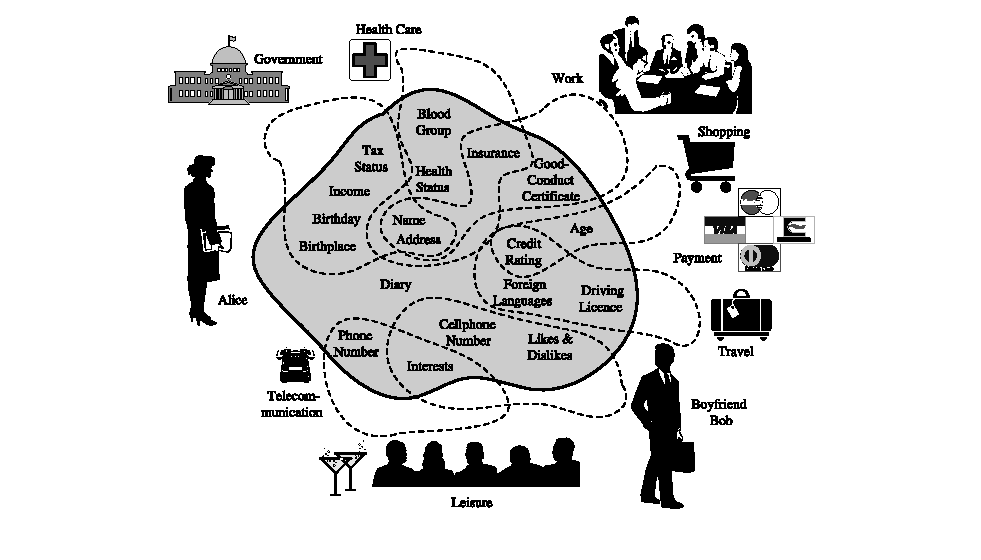
\includegraphics[width=\textwidth]{img/2_alice.eps}}
        \caption{Partial Identities of Alice extracted from \cite{claus_identity_2001}}
        \label{figure: alice}
    \end{figure}

    An important balancing act is to disclose the right amount of data to maintain anonymity, but also to provide the other person with the necessary information. For the purchase of a water, the kiosk vendor should not ask for any personal data, whereas verification of age when buying alcohol is a valid reason for information disclosure. In reality, official documents, such as state identification documents, or sometimes unofficial documents, such as customer cards, are usually used for such proof of identity. Here, users have full control over their documents as they are under their control, and only they can decide self-sovereignly whom and when to show them. Official identification documents are also produced and standardized to ensure the highest possible level of security and interoperability. Other countries can verify such documents without explicitly contacting authorities, simply by looking at the document. Confidence in the validity of the data arises from the fact that the verifying party trusts the authority issuing the document. \cite[p. 6]{struker_grundlagen_2021}

    As a result of the increasing digitalization of various branches of life, many processes are shifting to the digital world. Digital identities, which are similar to analogue identities in terms of their basic idea, are now being used for interacting with digital services. They allow entities, such as people or objects, to authenticate themselves online through certain attributes and thus prove their identity [\citealp[p. 103]{meinel_blockchain_2020}; \citealp{bundesdruckerei_so_2020}]. A more precise definition is given by Cameron \cite{cameron_laws_2005}, who defines digital identity as \textit{“A set of assertions that a digital subject makes about itself or another digital subject”}. In this context, a digital subject is \textit{“A person or thing represented or existing in the digital realm which is being described or dealt with.”} and the attributes mentioned can be represented in the form of claims, which are defined as \textit{“An assertion of the truth of something, typically one which is disputed or doubted”}. The problem is that analogue identities and their documents usually have no or not widely accepted \cite{krempl_e-government-studie_2019, koppenhofer_kabinettsbeschluss_2021} digital representations that could be used as a digital identity. From this emerged the patchwork of identity one-offs described in chapter \ref{chapter: ssi}, resulting in a divergence of digital identities from their original counterparts concerning their characteristics. To better understand this development, the next section describes the different stages of digital identities in more detail. [\citealp[p. 10]{struker_grundlagen_2021}; \citealp[p. 2]{ehrlich_self-sovereign_2021}]
    
	\section{Stages}
	
	As indicated in the last section, Allen's work \cite{allen_path_2016} has had a major influence on what is today considered Self-sovereign Identity and has been cited in over 100 works according to Google Scholar. According to him, digital identities, or online identities, have gone through four major stages since the beginning of the internet. These are examined in more detail below and show which developments led to the emergence of \ac{SSI}.
	
	    \subsection{Centralized Identity}
	    Centralized identities are identities that are issued and verified by a single party or hierarchy. The oldest examples of this are IANA (1988) for the administration of IP addresses, ICANN (1998) for domain names and \acfp{ca}, which play a major role today, particularly in connection with SSL certificates. Especially with the latter, the hierarchical structure of \acp{ca} becomes obvious when one looks at an SSL certificate in the browser. Here, a root authority allows another organization to manage its own hierarchy, while at all times the root authority has full control. This is highly critical for numerous reasons. For example, one entity has complete control over identities and can delete them at any time or even issue false identities. The latter can happen both willingly and unwillingly as a result of a hack. Due to the centralized nature of such authorities, they and thus also the complete hierarchy (chain of trust) are targets of attack, which has been shown in recent years \cite{borchers_diginotar-ssl-gau_2012}. Just like these organizations, due to the lack of an identity layer, all services on the internet developed similar centralized solutions (see chapter \ref{chapter: ssi}. This manifests itself above all in the various accounts that an internet user has to manage for various services. Again, users have little control over their data. \cite{allen_path_2016}
	    
	    \begin{figure}[ht]
    	    \centering
    	    \makebox[\textwidth]{\includesvg[inkscapelatex=false, width=0.6\textwidth]{img/3_central_schema.svg}}
            \caption{Relationship in centralized identities extracted from \cite[p. 7]{preukschat_self-sovereign_2021}}
            \label{figure: centralized}
        \end{figure}
	    
	    In addition, the user has to manage the abundance of login credentials efficiently and securely. However, it is also a challenge for the services, as they have to store a large amount of sensitive data securely and in compliance with data protection laws. Nevertheless, the beneficiaries here are the services, as they can act flexibly and independently of third parties and have full control over the data. \cite[p. 6]{ehrlich_self-sovereign_2021}
	    
	    
	    \subsection{Federated Identity}
	    
	    The second stage of development is represented by the so-called federated identities, which were intended to break down the hierarchies based on a single authority. Here, various commercial organizations developed a model in which control was to be divided between several federated authorities. One of the first projects in this area was Microsoft's Passport in 1999, where Microsoft created a single, federated identity for users that could be used on multiple sites. However, this unification came with the price that Microsoft was now at the center of the federation and could thus exert full control. Other efforts, such as Liberty Alliance Project, founded in 2001, attempted to create an actual federation between multiple companies in which control was distributed among them. The result, however, was a kind of oligarchy in which users still had no control over their data. In the end, the sites remained authorities. \cite{allen_path_2016}
	    
	    \begin{figure}[ht]
    	    \centering
    	    \makebox[\textwidth]{\includesvg[inkscapelatex=false, width=\textwidth]{img/4_federated_schema.svg}}
            \caption{Relationships in federated identities extracted from \cite[p. 8]{preukschat_self-sovereign_2021}}
            \label{figure: federated}
        \end{figure}
	    
	    Nevertheless, this type of digital identity is advantageous in that users do not have to manage an identity/ account for each service and companies have less administrative effort. The identity provider, e.g., Microsoft, acts as the issuer and owner of the data and is thus the central point of contact if a user wants to log on to another service of the federation. The user therefore has no control over his data and is dependent on the continued existence of the identity provider. Due to the abundance of sensitive data, it is possible for the identity provider \ac{IDP} to aggregate information from various areas in order to create user profiles, which in itself can lead to various problems. \cite[pp. 6 - 7]{ehrlich_self-sovereign_2021}
	    
	    \subsection{User-Centric Identity}
	    The goal of user-centric identity is to make federations obsolete and allow the individual to assert control over their identities across multiple authorities \cite{allen_path_2016}. The foundations for this, according to \cite{allen_path_2016}, lie in \cite{jordan_augmented_2003}, in which a \textit{persistent online identity} to be integrated directly into the architecture of the Internet was proposed, making federations unnecessary. One of their central demands was that users should have the right to control their own digital identity. This includes, among other things, the ability to decide what information is collected as part of their digital identity and who has access to which parts. Earlier approaches such as Microsoft's Passport or the Liberty Alliance Project were unable to meet these requirements because, as stated by \cite{jordan_augmented_2003}, they were too business-oriented and thus too focused on the privatization of information. According to them, everyone's digital identities should be a public good that should not be tied to the financial interests of a private company, as their commercial interest may not overlap with those of society. 
	    
	    These thoughts were guiding and influenced various future organizations and initiatives. One influential organization in this area has been the \acf{IIW}, which grew out of efforts by the Identity Commons and the Identity Gang. The \ac{IIW} community played a major role in shaping what is understood by user-centric identity and supported key standards such as OpenID (2005), OpenID 2.0 (2006), OAuth (2010), and OpenID Connect (2014). \cite{allen_path_2016} summarizes the focus of these efforts with the terms user consent and interoperability, which were non-existent or difficult to implement in previous models. These protocols have also been able to achieve significant success when considering the abundance of social logins from for example Facebook, Google, GitHub and Microsoft, which have taken a central position on various websites \cite[p. 8]{preukschat_self-sovereign_2021}. Nevertheless, the original approach of user-centric identities could not be realized further. Like in previous approaches, the identity data and thus absolute control remain with the \ac{SSO} providers who register them. \cite{allen_path_2016} mentions OpenID as an example, which theoretically allows users to set up their own OpenID providers. However, the complexity is so great that in reality this option is hardly ever used. Accordingly, the original problems that user-centric identities were supposed to solve could only be partially solved, since central, mostly private actors have maintained their authority over identity data. Fundamentally, user-centric identities are still federated identities that are now merely interoperable, which is why some literature \cite{ehrlich_self-sovereign_2021, preukschat_self-sovereign_2021} does not list them separately. \cite{allen_path_2016} 
	    
	    \subsection{Self-sovereign Identity}
	    \cite{allen_path_2016} refers to Self-sovereign Identity as the next and most current stage of digital identities, which is intended to solve the issues of all previous stages. In contrast to user-centric identities, users are not only at the center of the identity process, but should also be able to completely own and manage their identities. \cite[p. 12]{preukschat_self-sovereign_2021} describes this as a “[...] shift in control from the centers of the network [...] to the edges of the network [...]”, according to which all users interact directly with each other in a self-sovereign manner as peers. This evolution can be seen in figure \ref{figure: shift}. 
	    
	    \begin{figure}[ht]
    	    \centering
    	    \makebox[\textwidth]{\includesvg[inkscapelatex=false, width=\textwidth]{img/5_shift.svg}}
            \caption{Shift of control with \acs{SSI} extracted from \cite[p. 12]{preukschat_self-sovereign_2021}}
            \label{figure: shift}
        \end{figure}
        
        Apparent here is the new element \textit{registry}, which is used as a (decentralized) public key infrastructure \cite[p. 89]{preukschat_self-sovereign_2021}. A more detailed explanation of this is given in section \ref{section: standards}. To further describe the character of \ac{SSI}, \cite{allen_path_2016} defined 10 principles, with which he connects to previous works like the “Laws of Identity” by \cite{cameron_laws_2005}. These are:
        
        \begin{enumerate}
        	\item Existence: “Users must have an independent existence.”
        	\item Control: “Users must control their identities.”
        	\item Access: “Users must have access to their own data.”
        	\item Transparency: “Systems and algorithms must be transparent.”
        	\item Persistence: “Identities must be long-lived.”
        	\item Portability: “Information and services about identity must be transportable.”
        	\item Interoperability: “Identities should be as widely usable as possible.”
        	\item Consent: “Users must agree to the use of their identity.”
        	\item Minimalization: “Disclosure of claims must be minimized.”
        	\item Protection: “The rights of users must be protected.”
        \end{enumerate}
	    
	    SSI, according to \cite{allen_path_2016}, has its origins in the term “Sovereign Source Authority”, which originated in \cite{marlinspike_what_2012}. In this work, Marlinspike attributes to every human being the right to an identity, which is hindered by tight state structures. In the same year, work began on the Open Mustard Seed by Patric Deegan, which was intended to give users control over their digital identity in a decentralized system. This later resulted in the Windhover Principles (2014), under which the term Self-sovereign Identity appeared \cite{idcubedorg_id3_2014, hub_culture_hubid_2014}. These state, among other things, the following: \cite{allen_path_2016}
	    
	    \begin{displayquote}
            \textit{“Individuals [...] should have control over their digital identities and personal data ensuring trust in our communications, and the integrity of the data we share and transact with. [...] Individuals, not social networks, governments, or corporations, should control their identity credentials and personal data.”}
        \end{displayquote}
        
        Over the course of the following years, \ac{SSI} in connection with blockchain technology was frequently also being discussed in the \ac{IIW} community as well, and various ideas were being developed. This eventually led to some official agencies taking a closer look at this topic. For example, the U.S. Department of Homeland Security Science \& Technology division published a report in 2015 in which it addressed the previously discussed topics by the \ac{IIW}. The EU and countries such as China and Korea have also recognized the potential. In order to make \ac{SSI} implementable in reality, various new standards have been defined over the years in the W3C, among others, which will be discussed in more detail in the next section. \cite[p. 6]{preukschat_self-sovereign_2021}
        \vfill
	   
	% Four phases @Allen, add problems of those; types of identities, comparison
	\section{Standards}\label{section: standards}
	    In this section, an overview of various standards from different organizations is given. In addition, the two most important standards \textit{\ac{DID}} and \textit{\acf{vc}} will be discussed in more detail, as they are the basis for \ac{SSI} and various subsequent standards.
	    
	    \subsection{Overview}
	    \subsection{Decentralized Identifier}
	    % Zookos Triangle, Standard definition, did methods, did doc, lifecycle
	    \subsection{Verifiable Credentials}
	    % Lifecycles, 

		
	\section{Recent Developments}
		\subsection{DIDComm}
		\subsection{Zero Knowledge Proofs}
		\subsection{RevocationList2020}
	
	\section{Architecture}
	\subsection{Roles}
	\subsection{Components}
% work in progress

\chapter{Expert Questionnaire}\label{chapter: expert}

	\section{Expert Selection}
	
	\section{Questionnaire}
	\subsection{Solutions Overview Draft}
	\subsection{Questions}

	\section{Results}
	
	
\chapter{Reference Implementation}\label{chapter: implementation}

This chapter focuses on the development of a reference implementation covering the \ac{vc} lifecycle, which is based on learnings of the last few chapters concerning theoretical background and opinions of experts. It is intended to directly address the lack of practical considerations of \ac{SSI} solutions in the research area, by leveraging four of the previously listed solutions that can be used to implement the \ac{vc} lifecycle. In the next sections, the complete implementation process will be described, starting with preliminary considerations and ending with results and lessons learned.

    \section{Considerations}\label{section: ri-considerations}
    % Considerations: What should be done? Why? What's important? What not? Which implementations have i chosen? Which language for reference implementation? Why API?
    As previously stated, the reference implementation should exemplarily implement four solutions in such a way that they map, based on their capabilities, the \ac{vc} lifecycle as much as possible. This enables a practical validation of the promises made by the solution providers and can thus provide a thorough insight into the existing or missing range of functionality. This way, possible blind spots or even insufficient features can be identified, which can be used to further improve the available solutions. This approach can additionally generate added value for developers who want to use \ac{SSI} technologies in their projects, since actual experiences, capabilities, and code of the individual solutions can be reused from a real implementation process.
    
    Since the results of the implementation are also to be incorporated directly into a new developer-oriented evaluation framework, there are some key considerations that must be defined beforehand. To meet the objectives described in this section, the following considerations were established:
    % Maybe add something along the lines of: MVP -> i don't care about error handling and edge cases
    \begin{itemize}
        \item \textit{Use-case agnostic}: In order to represent the \ac{vc} lifecycle as broadly and standardized as possible, the reference implementation should not be bound to the requirements and specifics of a use case. Focusing on a specific use-case could possibly lead to certain parts of the \ac{vc} lifecycle being underrepresented or not implemented at all. Such an open approach can also invite a closer look and implementation of specific facets of a technology that would have been unnecessary for a use case. This also means that the reference implementation must be accessible in such a way that it can be used relatively independently of the technology stack being used for a use case.
        \item \textit{Flexible architecture}: The reference implementation should leverage a software architecture that makes it as easy as possible to plug in new \ac{SSI} solutions. Peculiarities and complexities should be abstracted away to create a flexible and resilient architecture. 
        \item \textit{Community efforts} Since the \ac{SSI} community is very active, it should be checked beforehand which previous work can be reused for the implementation. This applies to both the architecture and the software libraries used. In this way, it can be ensured that the work does not disregard the requirements of the community and thus reality.
        \item \textit{Implementation experience}: Throughout the entire development process, objective experiences and findings should be documented and summarized. As already mentioned, these may be relevant for other developers, the solution providers, and also for the mentioned evaluation framework.
    \end{itemize}
    
    Taking these four points into account, the goal is to create a reference implementation that is as helpful as possible. The next section explores this, starting with the base implementation and community efforts to date, on which further work can be based on.
    
    \section{Base Implementation}\label{section: base-implementation}
    % Basis for Implementation: vc-http-api -> why? What is it for? What changes/ additions have to be made? Why can I hijack it? API Document!
    % Technical basis -> express app, typescript 
    A RESTful API was chosen as the basic implementation form, since it is technology-independent and can be used in various programming languages and environments. It is only necessary that HTTP requests can be sent, which allows a high degree of flexibility in later applications. 
    
    As a basis, this work is roughly based on the ideas of the W3C Credentials Community Group, which has created an unofficial draft API definition called “Verifiable Credentials HTTP API”. This describes the structure of an API with all its routes, request, as well as response bodies, which can be used for the \ac{vc} “lifecycle management”. The group defined API contracts according to the OpenAPI standard, which were originally intended to be used as a basis for verifying interoperability of \acp{vc} issued by different providers (see interoperability report from \cite{homeland_security_preventing_2020}). It is important to note that the reference implementation is based on the state of the API contract as of April 2020 (v.0.0.2-unstable), as some small things have changed since then. The contract is strongly based on the \ac{vc} standard and divides the API into resources for the three roles: Issuer, verifier, and optional holder. The includes resources for issuing and verifying \acp{vc} and \acp{VP}, deriving, as well as revoking \acp{vc}. At this point, it should be emphasized again that this is an API definition and not an actual implementation. \cite{world_wide_web_consortium_credentials_community_group_vc_2021, world_wide_web_consortium_credentials_community_group_verifiable_2021}
    
    With regard to the reference implementation, this preliminary work is quite helpful, even if it doesn't fully cover the whole \ac{vc} lifecycle. Therefore, some changes and additions have been made. A graphical representation of the API definition is shown in Figure X, which also allows testing of the individual routes.
    \newpage
    \begin{figure}[ht]
        \centering
        \makebox[\textwidth]{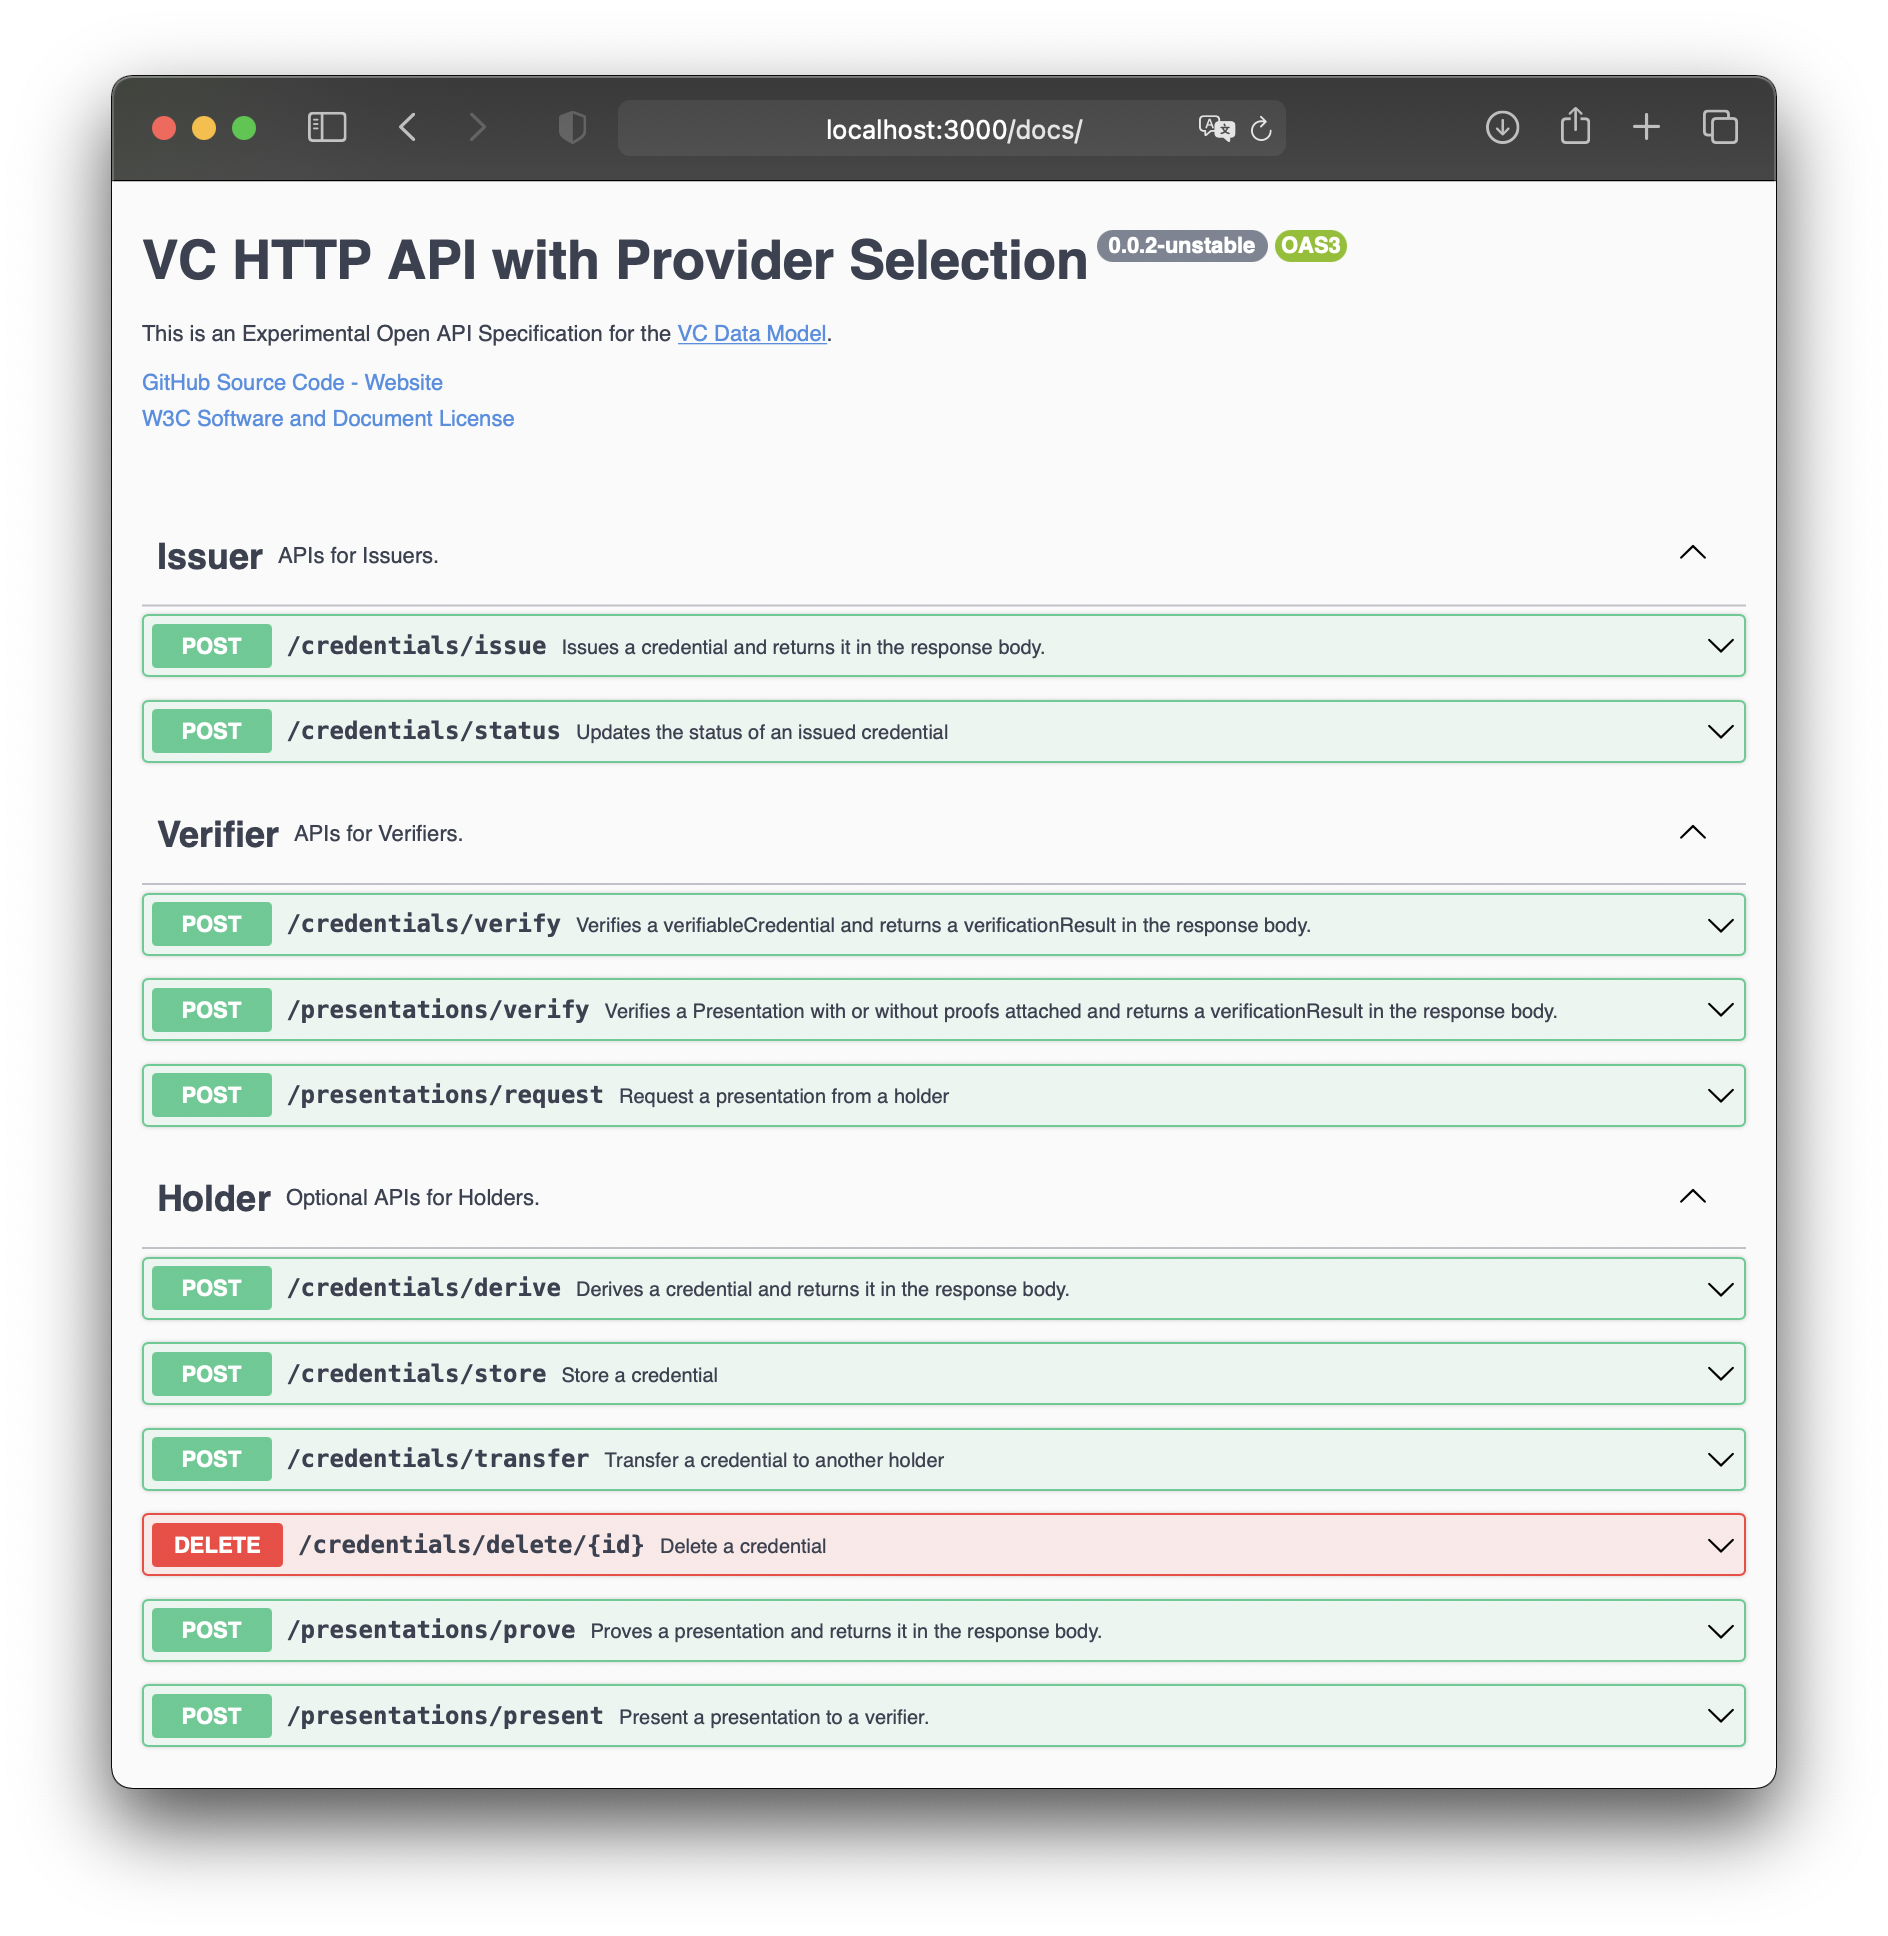
\includegraphics[width=0.9\textwidth]{thesis/img/13_api_definition.png}}
        \caption{Modified API definition (based on \cite{world_wide_web_consortium_credentials_community_group_vc_2021})}
        \label{figure: api definition}
    \end{figure}
    
    All changes made to the original definition are summarized by the following points:
    
    % TODO: might be incomplete 
    \begin{itemize}
        \item \textit{Provider selection}: Since four solutions should be addressable via the API, a query parameter was added to each route, which is based on a custom provider schema definition. Thus, it is possible to specify which solution/ provider should handle a request.
        \item \textit{Destination selection}: Another query parameter allows defining whether a request has the local or a remote agent as target. This mainly includes the issuing route for a \ac{vc}, which allows a \ac{vc} to be sent directly to the subject's agent or imported via QR code. In other cases, such as transferring \acp{vc} or presenting or requesting presentations, can be done directly via the request body. For this purpose, the schema \texttt{GenericMessage} was defined, which in its structure is very roughly based on the DIDComm data model.
        \item \textit{Added routes}: To complete the lifecycle coverage, a route to create a presentation request has been added to the Verifier and routes to save, delete, transfer of \acp{vc} and presenting \acp{VP} have been added to the Holder. For the request and response bodies, existing schemas were reused as much as possible.
        \item \textit{Response bodies}: Since some response bodies contained too much information for the requirements of the API, the schema \texttt{GenericResult} was introduced, which only contains whether the operation was successful and whether there were errors. This is the case for verifying, storing, deleting, and transferring \acp{vc} and verifying, as well as requesting/ presenting \acp{VP}.
    \end{itemize}
    
    The goal of the customizations was to ensure that the original API definition did not constrain the implementation, while retaining fundamental parts of the community work. 
    
    Based on the expert survey and observations from the IIW April 2021, the solutions Veramo from ConsenSys Software Inc, MATTR VII from MATTR Limited, Trinsic Core from Trinsic Technologies Inc, and Azure AD Verifiable Credentials from Microsoft were selected as the four solutions to be included in the reference implementation. For the implementation language, TypeScript was chosen as it was the only language where Veramo, Trinsic and Azure offer SDKs for. In addition, other basic libraries in the \ac{SSI} area are written in TypeScript or at least JavaScript and would thus integrate more easily into the implementation to possibly add missing features. Unlike JavaScript, various features of TypeScript allow cleaner and more robust code \cite[p. 87]{zammetti_modern_2020} that can simultaneously benefit from much of the existing JavaScript packages being made available from the open-source community.
    
    Building on this decision, node.js was selected as the JavaScript runtime that can be used in combination with the express.js library to develop highly scalable web applications such as APIs \cite{openjs_foundation_about_2021, openjs_foundation_express_2021}. To make TypeScript work in this environment, various dependencies such as TypeScript, ts-node, eslint, and some type definitions were installed via the Node Package Manager. The next section describes how these components and the four solutions were combined into a flexible software architecture.
    
    \section{Architecture}\label{section: architecture}
    % Software architecture, factory method pattern -> why? Describe how solutions tap into it.
    
    With regard to the considerations in section \ref{section: ri-considerations}, the factory method design pattern was chosen for the software architecture. It belongs to the creational patterns and thus influences how the instantiation process is carried out. A developer can thus decide independently of the system how, for example, objects are created, which enables a high degree of flexibility. It defines an interface or an abstract class for the creation of objects, whereby the instantiation of objects is done by subclasses instead of a class. This is useful, for example, if a class does not yet know which objects it needs to create at runtime. \cite[pp. 81, 85, 107-108]{gamma_design_1995} 
    
    This is pattern is appropriate because a request determines which solution and thus which objects have to be created. In addition, it allows the complexities of the individual solutions to be abstracted away, so that when defining the individual routes, only the concrete factory class must be called, which returns the correct object of the requested solution. This way, the routes only need to be programmed once and additional solutions can be added afterwards without having to change the code of the routes. Figure \ref{figure: factory method} shows a UML diagram that represents the concrete factory method pattern in the reference implementation. The interface \texttt{Factory} defines a method \texttt{createProvider()}, which is implemented by the class \texttt{ServiceProviderFactory}. This is the class which is instantiated, for example, in the routes and which is used to retrieve the object of a provider. A provider is the class of one of the four solutions that implements basic methods like the \ac{vc} issuance defined by the \texttt{ServiceProvider} interface.
    
    \begin{figure}[ht]
	    \centering    	    \makebox[\textwidth]{\includesvg[inkscapelatex=false, width=0.8\textwidth]{img/14_uml_ref.svg}}
        \caption{Factory method pattern in reference implementation (extracted and edited from \cite[p. 107]{gamma_design_1995})}
        \label{figure: factory method}
    \end{figure}
    
    A second pattern, which was integrated, is the Singleton design pattern. This is used in the individual concrete provider classes and allows that only one globally callable instance of a provider class can be created \cite[p. 127]{gamma_design_1995}. The rationale for this is that no more than one object is needed, caching is simplified, and multiple provider objects could lead to unforeseen complications.
    
    Looking at the complete system architecture, the previously described software architecture integrates tightly. The service provider factory sits between the routes for issuer, verifier, and holder and the concrete classes of the individual providers. Its features in the architecture can be summarized as follows and can be seen in Figure \ref{figure: sys architecture}:
    
    \begin{itemize}
        \item \textit{Veramo Provider}: The provider class requires an agent class from Veramo, which enables the integration of extensions for various functionalities. This can be, for example, the Uniresolver for resolving \acp{DID} or various services with which a connection to blockchains can be established for various actions (e.g. Infura or Microsoft's Anchoring Service). The agent also offers a REST API, which allows any actions to be executed from a remote location. Furthermore, the agent can connect to other Veramo agents on the Internet and, for example, exchange messages of any kind via DIDComm or resolve their \acp{DID}. A more detailed explanation of Veramo can be found later in subsection \ref{subsection: veramo}.
        \item \textit{MATTR Provider}: This provider communicates directly with the MATTR API, which handles any operations. Additionally, there is a callback service between the API and the provider, which can receive verification results from the MATTR platform, e.g. triggered by scanning a QR code through a mobile wallet.
        \item \textit{Trinsic Provider}: Similar to the MATTR provider, this also communicates directly with the Trinsic API and a callback service catches verification results. Thus, as with MATTR, the actual \ac{SSI} logic is outside the reference implementation.
        \item \textit{Azure Provider}: This provider is integrated into the architecture similar to MATTR and Trinsic. 
    \end{itemize}
    
    \begin{figure}[ht]
        \centering
        \makebox[\textwidth]{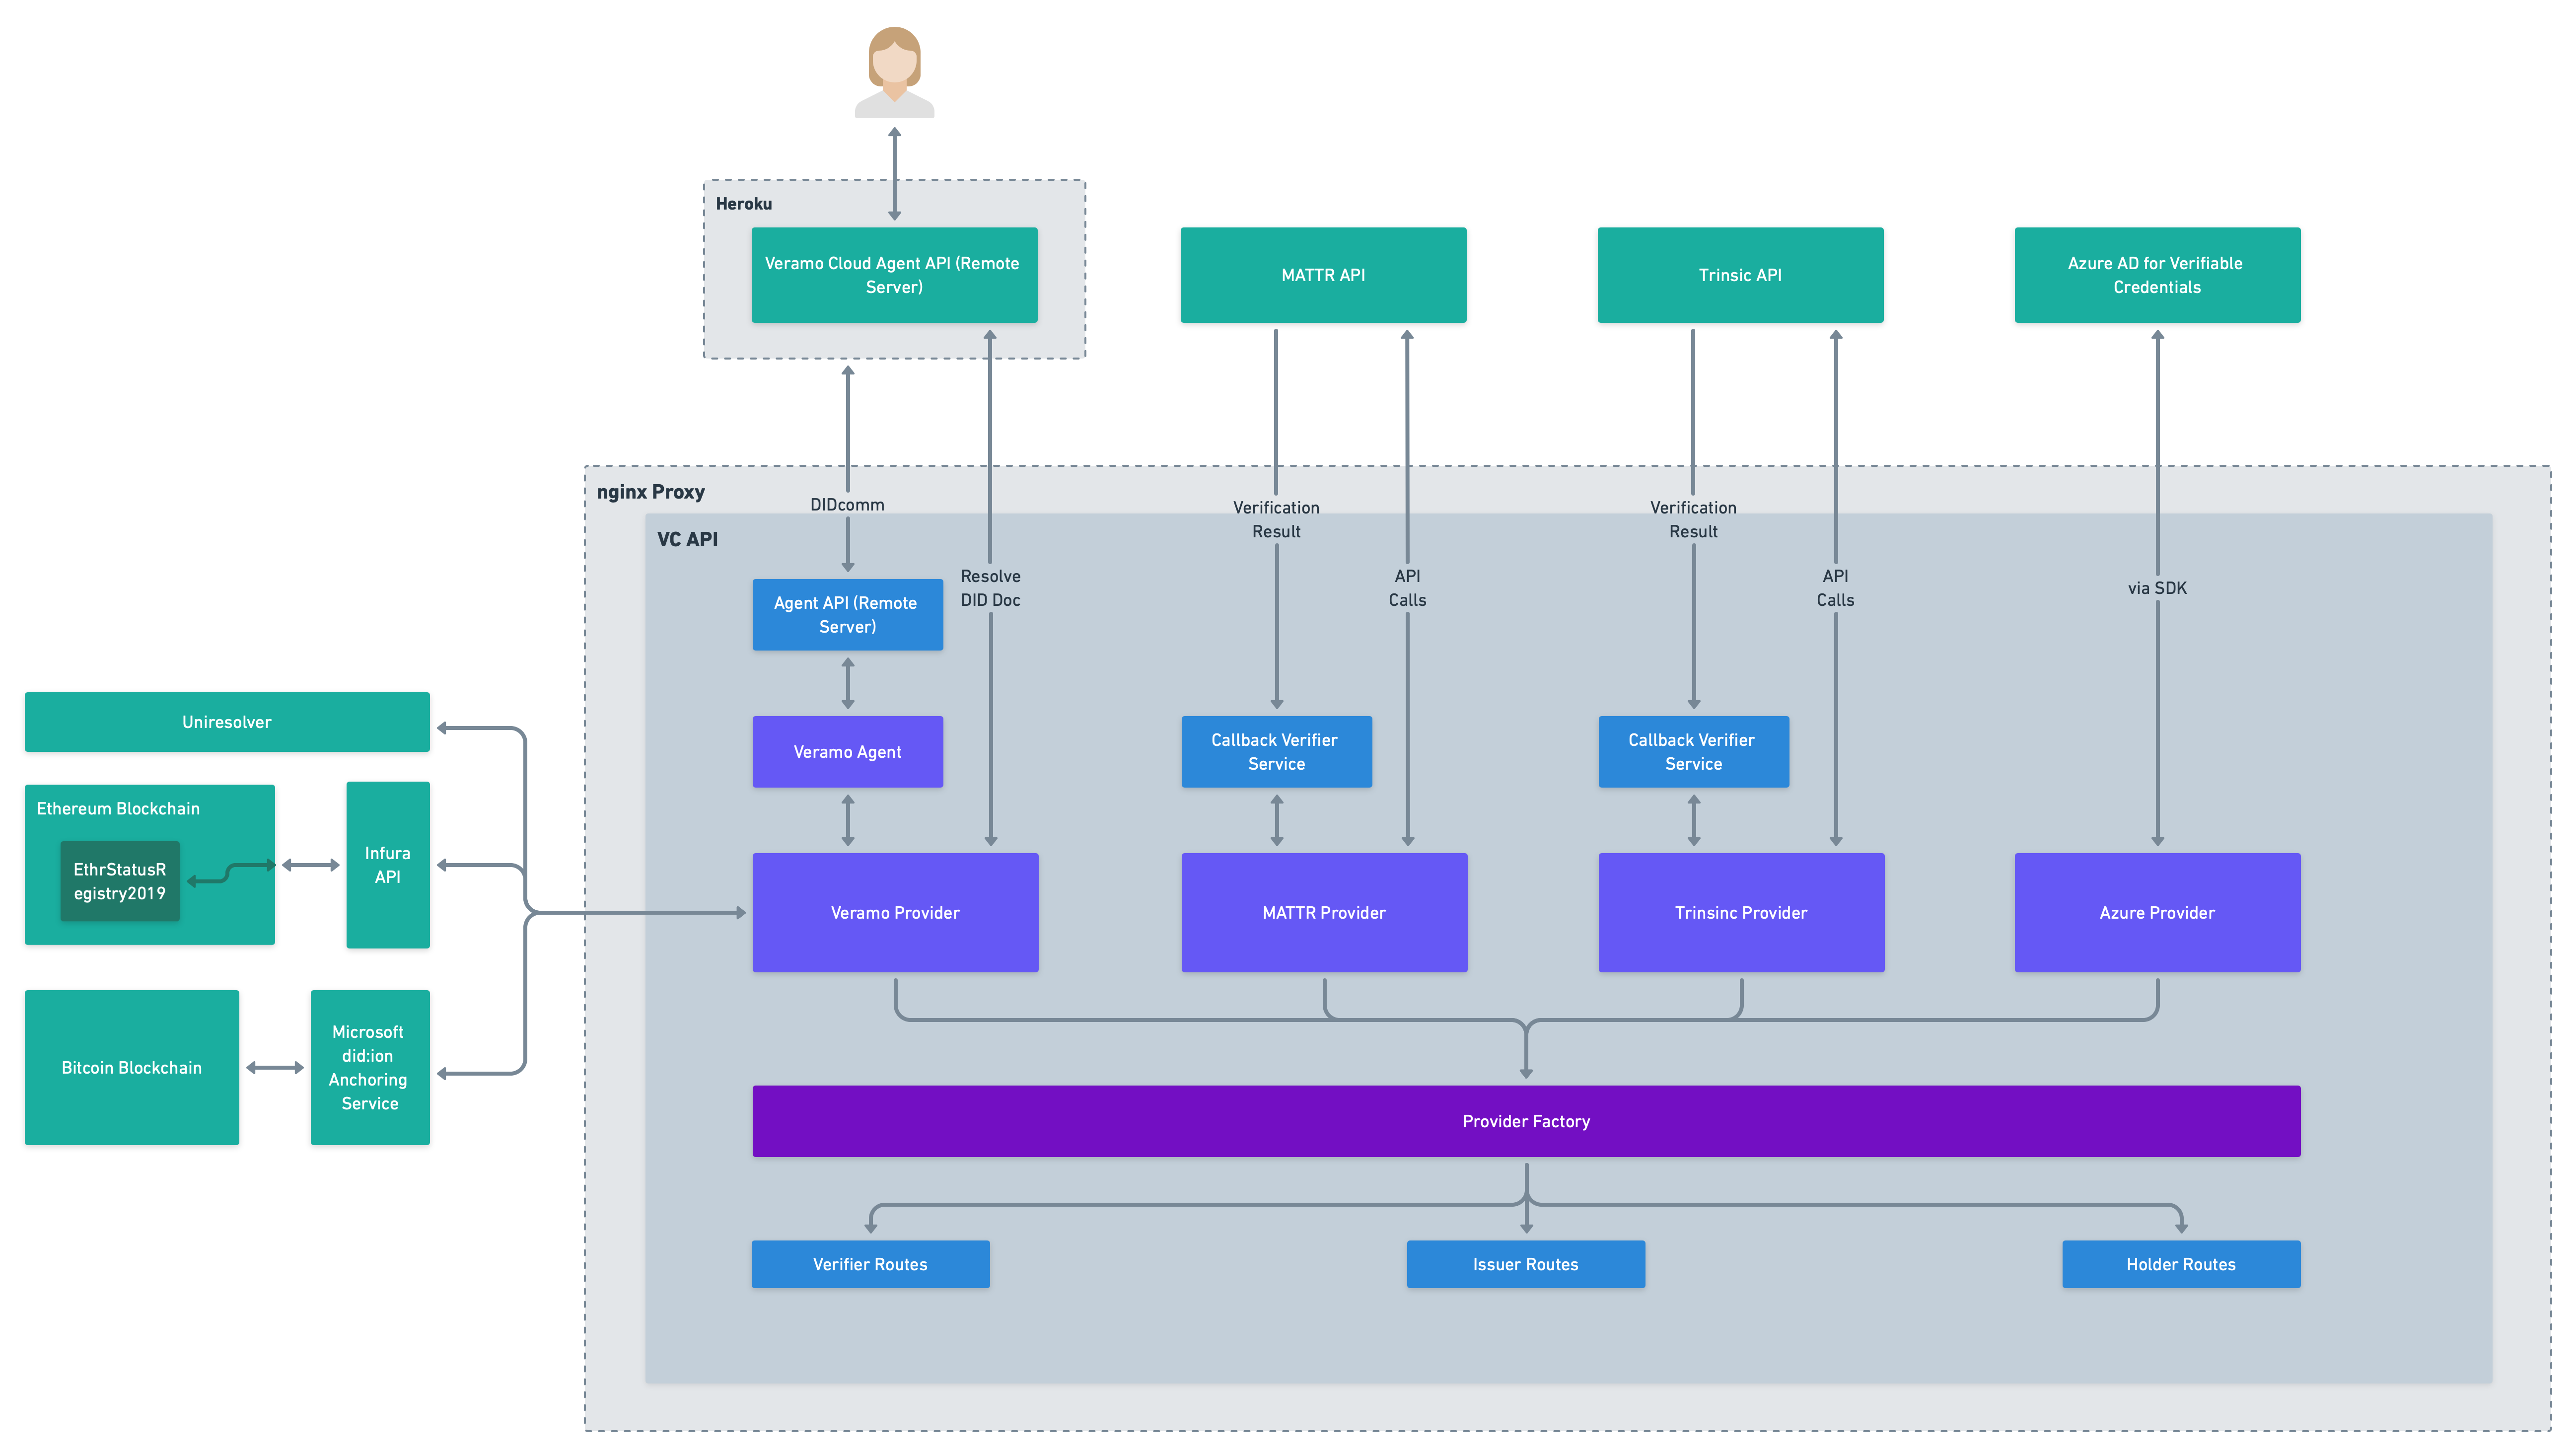
\includegraphics[width=\textwidth]{thesis/img/15_architecture.png}}
        \caption{System architecture}
        \label{figure: sys architecture}
    \end{figure}
    
    \vfill
    
    \section{Solution Integration}\label{section: integration}
    % Describe implementation process, what has been done, what not. What worked, what not? What was problematic? What did I like?
    \subsection{MATTR}\label{subsection: mattr}
    \subsection{Trinsic}\label{subsection: trinsic}
    \subsection{Veramo}\label{subsection: veramo}
    \subsection{Azure AD}\label{subsection: azure}
    \section{Results}\label{section: ri-results}
% work in progress

\chapter{Evaluation Framework}\label{chapter: framework}

    Allgemeiner Einstieg; Warum noch mal eval frame? Ziel.

	\section{Requirements}
	
	Grundlegende Anforderungen -> developer focus, was soll abgebildet werden (siehe implementierung, umfrage)
	
	\section{Criteria \& Questions}
	
	Prozess: Grundlegende Bereiche/ Kategorien definieren (als Frage), definieren der Kriterien -> Fragen
	
	Darstellung in Tabellenform
	
	Punktevergabesystem
	
	\section{Results}
	
	Einordnen der Lösungen in Tabelle -> Bewertung
	
	Was sind die Ergebnisse? Welche Lösung eignet sich für das? Was machen welche Lösungen sehr gut, sehr schlecht? Überraschungen bezügluch Vorbetrachtung?
	
	
\chapter{Conclusion}

%Digital identities und ihre Umsetzungen sind ein Jahrzente altes Problem, was bisher nur unzureichend gelöst werden konnte. Aktuelle Ansätze führen zu noch nie da gewesenen Leaks persönlicher Daten und dem Verlust von Kontrolle über von Millionen von Menschen weltweit.

Self-sovereign Identity is a new approach towards digital identities. This thesis gives an overview over existing developer-oriented \ac{SSI} solutions and defines a new approach to evaluate them. For this purpose, an evaluation framework based on expert interviews, practical experience and the \ac{vc} lifecycle was developed, which enables an objective and structured evaluation of such solutions. At the same time, this work closes a gap in the existing literature. With a few exceptions, the literature has so far only focused on fundamental research and less on practical considerations of existing solutions.

For the described artefacts, further research and an expert survey were used to create an overview of various solutions on the market and their capabilities to cover the \ac{vc} lifecycle. A total of seven experts from the \ac{SSI} space who work on standards, open-source libraries and commercial solutions took part in a questionnaire and generated input for chapters \ref{chapter: expert} and \ref{chapter: framework}.
The expert input helped improve the research on 15 solutions across four categories (RQ1):
\begin{itemize}
    \item Platforms: Mattr, Trinsic, Azure AD for \acp{vc}, Verity, Affinidi
    \item SDKs: Dock.io, aca.py, Jolocom
    \item Frameworks: Veramo
    \item Libraries:  DIDKit, TangleID, Identity.com, vc.js, vc-js, verifiable-credentials-java
\end{itemize}
Among them, the solutions Mattr and Trinsic received most of the recommendations with 3 out of 7 votes in the questionnaire (RQ2).

In addition, a new developer-oriented evaluation framework based on expert opinions and practical experience was developed. For this purpose, experts were asked about important selection criteria for \ac{SSI} solutions. Moreover, a reference implementation integrating four of the solutions was developed and described. This resulted in the five categories functionality, flexibility, operability, dependency, and involvement. These in turn contain a total of 15 individual criteria, corresponding questions and a scoring scheme for a practical evaluation. For the implemented solutions Mattr, Trinsic, Veramo and Azure, Veramo received the highest score with 76.75\% and Azure the lowest with 43.78\% without weighing the individual indexes. (RQ3)

In summary, this work is the first to describe a developer-oriented examination, implementation, and evaluation of solutions in the \ac{SSI} domain. With some solutions, the concepts and technologies of \ac{SSI} can already be integrated in a production-ready manner, but the relatively young field and consequently the partially unfinished standards are still a hindrance for many solutions. In addition, it should be observed that platform solutions do not create centralized data silos and unnecessary dependencies. This would again create similar issues and situations that \ac{SSI} was meant to solve.





%Literaturverzeichnis
\newpage
\lhead{}
\rhead{\leftmark}
\addcontentsline{toc}{chapter}{Bibliography}
\bibliography{references}

\appendix

\appendix
\chapter*{Appendix}\label{chapter: appendix}
\markboth{Appendix}{}

\section*{A Conversation with Orie Steele}\label{appendix: steele}
\begin{Verbatim}[breaklines=true, breaksymbol={}, breaksymbolsepleftnchars=2]
From: Orie Steele
To: Philipp Bolte

1. What is your job title? (Developer, Researcher, ...)
CTO of a Verifiable Credentials and Decentralized Identifiers as a service company.
 
2. Are you currently working on anything SSI-related?
> Applications of VCs and DIDs to physical and software supply chain.
 
3.What fascinates you about SSI?
> Applications of cryptography that enable better control of digital space for both humans and machines / companies.
 
4. What value would you attribute to the experience of a developer concerning its available toolset for the successful implementation of SSI products?
> Reinventing the wheel / building on non standard or draft level crypto is a major barrier to adoption.
 
5. Looking at the spreadsheet, what additions or changes would you make?
You need some measure of interoperability, for example, store and transfer may be only limited to certain credential formats.
 
6. If you were a developer at a company looking to integrate Verifiable Credentials into their products, which three solutions would you look at and why?
> I'm biased, but I like the approach transmute, trinsic and didkit are taking, building APIs that can be proved interoperable from the start.
 
7. Which ones wouldn't you use and why?
> Too early to not look at any of them, but I would object to any that claimed that only 1 format or one protocol was going to work for everything... 
which historically Microsoft and Evernym have associated with... but both are changing.
 
8. What do you consider essential criteria for selecting a good SSI solution for implementing Verifiable Credentials?
> Proven interoperability and portability. Open contribution to standards. 
 
9. What do you think are common problems existing SSI solutions for developers have? 
> Over focus on crypto that is not well supported.  Too much attention on people, not enough attention on businesses and devices.
 
10. Is there something you still want to say?
> I would love to see the results of this, when you gather more feedback.

OS
\end{Verbatim}

\section*{B Conversation with Martin Riedel}\label{appendix: riedel}
\begin{Verbatim}[breaklines=true, breaksymbol={}, breaksymbolsepleftnchars=2]
From: Martin Riedel
To: Philipp Bolte

Lieber Herr Bolte,

vielen Dank für Ihr Interesse und es freut mich, dass Sie IIW verfolgt haben (ja aktuell leider nur remote…). Gerne beantworte ich Ihre Fragen (siehe Inline).

Ich wünsche Ihnen alles Gute für Ihr weiteres Studium.
Martin Riedel

1. What is your job title? (Developer, Researcher, ...)
> I somehow self-assigned “Identity-Engineer” as a title. Not sure if it will catch on though, since it might get confused with some self-improvement business model :)

2. Are you currently working on anything SSI-related?
> Yes, I work for Consensys, an Ethereum Software House. I’m concentrating my work on Product Management and Development of Veramo, as well as some R&D related topic like DID-method Scaling (Developing a DID method based on ZK-Rollup Technology)

3. What fascinates you about SSI?
> As a German I’m naturally very conscious around privacy and data-security in general. I often try to interpolate how the Internet would look in X years if we keep going down the same road of online monopolies ingesting and monetizing our personal data. (Answer: It’s not good.) We need a perspective shift to keep and open and private Internet and SSI is the single most important element to archive this.

4. What value would you attribute to the experience of a developer concerning its available toolset for the successful implementation of SSI products?
> Implementing an identity-stack end to end is a hard problem and there are numerous pitfalls in doing so. That’s why I personally am supportive of SDKs and frameworks that abstract most of the technical complications from a developer. Veramo is one of those, but there are numerous others. Even purpose-build SSI frameworks need to rely on fundamental crypto-libraries in order to provide secure signing, verification, encryption and proofing capabilities. Since any single mistake can threaten the privacy and sovereign aspects of an SSI ecosystem it is very important to rely on well-tested base frameworks and libraries.

5. Looking at the spreadsheet, what additions or changes would you make?
- Credential Status Check do not necessarly make it “home” to the issuer. “Phone-home problem”. That what ZKP-based Proofs (e.g. using Accumulators on a Blockchain) try to solve.
- In Regard to Veramo: 
	- Veramo offers a Datastore Layer Interface to store and retrieve. DIDComm Messages, unwrapped Verifiable Presentation, unwrapped Verifiable Credentials (https://github.com/uport-project/veramo/tree/next/packages/
	data-store)
	- Generally I would probably argue that Store and Delete of SSI Data might not even be a core problem of the credentials flows. (E.g. is data stored locally or in some kind of hosted EDV service is up to the specific architecture design)
	
6. If you were a developer at a company looking to integrate Verifiable Credentials into their products, which three solutions would you look at and why?
> Veramo, Aries (Go, AcaPy), Identity.com (Civic)

7. Which ones wouldn't you use and why?
> (Pure) Indy-based implementations / Anoncreds v1 (because of the known limitations around their proving limitations and  non-conformant VC/VP structure)

8. What do you consider essential criteria for selecting a good SSI solution for implementing Verifiable Credentials?
- Full interoperable Support of current DID-Core and VC specs
- Interoperable Showcases
- Language-support for the implementation of my choice
- Thought leadership of the creators in the space

9. What do you think are common problems existing SSI solutions for developers have? 
- Choosing the right framework while the community is still solving interoperability showcases. 
- Implementing a solution that protects the privacy of each participant. (Even if SSI Framework X provides the perfect Hammer for the problem, you can still very much use it in the wrong way).

10. Is there something you still want to say?
> Good to see that this space is getting traction in academia as well! I hope the EU will the a leader in supporting (and also funding) this technology to protect it’s citizens from big internet data monopolies.
\end{Verbatim}

\section*{C Conversation with Riley Hughes}\label{appendix: hughes}
\begin{Verbatim}[breaklines=true, breaksymbol={}, breaksymbolsepleftnchars=2]
From: Riley Hughes
To: Philipp Bolte

Thanks Philipp. See answers inline.

Riley Hughes

1. What is your job title? (Developer, Researcher, ...)
> CEO, cofounder

2. Are you currently working on anything SSI-related?
> Yes, we're an SSI platform

3. What fascinates you about SSI?
> It reduces transaction costs for people to engage w/ others & access things they need

4. What value would you attribute to the experience of a developer concerning its available toolset for the successful implementation of SSI products? 
> I'm not sure if I understand the question... but I can say that developer experience is critical, not just for the implementors, but also to get others in an ecosystem to adopt credentials, it needs to be easy to implement.

5. Looking at the spreadsheet, what additions or changes would you make?
> I don't see a spreadsheet

6. If you were a developer at a company looking to integrate Verifiable Credentials into their products, which three solutions would you look at and why?
> I would look at Trinsic #1 of course 
:) after that, Mattr and Microsoft

7. Which ones wouldn't you use and why?
> I wouldn't use open source repos, because of the maintenance and overhead of building and maintaining it in-house. I'd want to focus on the product we're developing. I also wouldn't use tools from companies focused on IAM, unless my SSI use case was strictly IAM, in which case I'd only use these tools (IdRamp, esatus, etc)

8. What do you consider essential criteria for selecting a good SSI solution for implementing Verifiable Credentials? 
> How long will it take me to implement? And how long will it take others in my ecosystem to implement? (e.g., if I'm a university, how long will it take employers, HR providers, other universities, etc to accept the creds I issue? If they're not accepted anywhere it's pointless.)

9. What do you think are common problems existing SSI solutions for developers have? 
> There is always a balance between being opinionated about implementation to abstract away complexity, or exposing complexity to be more flexible. It's challenging to strike a balance between those.

10. Is there something you still want to say?
> It's all about the ecosystem. No single company will implement SSI just for themselves. That is why interop & ease of impl, etc are so important.

    From: Riley Hughes
    To: Philipp Bolte
    
    Just saw the spreadsheet. I would add trinsic is platform + SDK. also, last I checked Evernym didn't support revocation, but maybe you have more recent data than me. But revocation isn't all created equally - privacy factors and scalability are important considerations (ie, it might be better to support no revocation, than support a scheme with bad privacy). Finally, for transferability, i'm not sure what you mean, but you can see this blog post and maybe it answers your quesiton: https://trinsic.id/ssi-digital-wallet-portability/

        From: Philipp Bolte
        To: Riley Hughes
        
        [...]
        Thank you for bringing up the blog post. I attached explanations from the w3c specs to the bottom of the spreadsheet. And they say „A holder might transfer one or more of its verifiable credentials to another holder.“  To me it rather sounds like a transfer of VCs between subjects (no presentation, verification) than portability, which is important as well though. Or am I misunderstanding that?
        
        Again, thank you very much and have a great week!
        
        Philipp Bolte

            From: Riley Hughes
            To: Philipp Bolte
            
            We don't support transporting credentials from one subject to another. The only way we would support that is if it were auditable so you could tell the audit trail of transfers, but that is not on the immediate roadmap for anyone in the space that I'm aware of.
            
            You have a great week as well :-)
            
            Riley Hughes
\end{Verbatim}

\section*{D Conversation with Markus Sabadello}\label{appendix: sabadello}
\begin{Verbatim}[breaklines=true, breaksymbol={}, breaksymbolsepleftnchars=2]
From: Markus Sabadello
To: Philipp Bolte

Sehr geehrter Herr Bolte,

Tut mir leid für die späte Antwort.

Hier meine Antworten:

1. CEO at Danube Tech (https://danubetech.com/)

2. Yes, I am working on a lot of SSI projects, e.g. the DIF Universal Resolver, the W3C DID Core 1.0 specification, the E.U.'s ESSIF-Lab program, the U.S.' DHS SVIP program, as well as multiple software libraries and other community projects.

3. The most fascinating part about SSI is that is not only a technical solution, it also asks deep political and philosophical questions about the nature of humans, about their freedom and sovereignty.

4. I don't really understand the question. :( I think there are a lot of useful toolsets for developers, but it might also be confusing since not all are fully interoperable with one another.

5. I would add verifiable-credentials-java, which was one of the earliest implementations of Verifiable Credentials. You could also add the Universal Issuer and Universal Verifier.

6. I would use our own implementation verifiable-credentials-java :) But I would also recommend vc-js (Digital Bazaar), DIDKit, and Veramo.

7. I think personally I wouldn't use Azure AD, Identity.com credential commons, Evernym (Verity-sdk, Connect.me), Trinsic, since those feel a bit too corporate and "locked in".

8. The most important criterium is how involved the leaders of a particular SSI solution are in community organizations and processes.

9. The most common problems are probably that specifications and protocols are still changing rapidly, and that a lot of solutions are not as interoperable with one another as they should be.

10. Thanks for your work.. Research like yours is super valuable to make SSI solutions more accessible!

Markus

    From: Philipp Bolte
    To: Markus Sabadello
    
    Sehr geehrter Herr Sabadello,

    vielen lieben Dank für Ihre Antwort. Frage vier ist tatsächlich etwas unglücklich formuliert. Letztendlich wollte ich damit Meinungen erhalten, wie wichtig die Developer Experience (analog zu User Experience zu verstehen) ist, bezogen auf vorhandenes Toolset und Werkzeuge wie SDKs. Darin enthalten sein kann z.B. ease of use, completeness & understandability of documentation, …
    Weil in der Literatur und auf diversen Meetups wird häufig über die User Experience gesprochen, obwohl eine gute Developer Experience in meinen Augen mindestens genauso wichtig ist, damit gute SSI-enabled Products auf den Markt kommen. Könnten Sie eventuell noch einen angepasst Antwort nachreichen? 
    
    Viele Grüße
    Philipp
        
        From: Markus Sabadello
        To: Philipp Bolte
        
        Ah jetzt verstehe ich es, danke für die Erklärung :) 

        Ich würde sagen:
        
        4. Developers don't like to read long technical specifications and documentation. It is very important for developers to be able to get started quickly, with simple tutorials and - most importantly - examples that they can use as a starting point for their own projects. Another critical aspect for developers is how quickly they can get support e.g. via Github issues or regular community meetings where questions can be asked.
        
        lG
        Markus Sabadello
\end{Verbatim}

\section*{D Conversation with Stefan Adolf}\label{appendix: x}
\begin{Verbatim}[breaklines=true, breaksymbol={}, breaksymbolsepleftnchars=2]
From: Stefan Adolf
To: Philipp Bolte

Hey Philipp,

hier kommen ein paar Antworten :) Schönes Wochenende!

1. What is your job title? (Developer, Researcher, ...)
> I'm "Developer Ambassador" at Turbine Kreuzberg which is a union of a fullstack development job, technical and public writing and communication / community building tasks.

2. Are you currently working on anything SSI-related?
> absolutely. We're evaluating the space by building Proof of Concepts for immunization credentials. We as well have built prototypes using fully trustless libraries (3box which is deprecated now) and are in close contact with some major players (e.g. Jolocom, Main Incubator, ceramic). Turbine Kreuzberg is an application development service company and not a technology driver in that sense: we're trying to figure out what's going to be a requirement for our customers in the near future and implement solutions for them along services we find to be suited for each case.

3. What fascinates you about SSI?
> getting rid of federated login systems and centralized profiling is one thing - the idea that few companies own all my information and are able to correlate at will is quite intimidating. I like the idea that by just using cryptographic primitives and adding trust anchors I can start trusting people - and thanks to the 2020s tech stack it's quite useable. On the other hand SSI will allow us to connect official endpoints in a privacy preserving way without the need to disclose anything besides what's needed. That's going to revolutionize the way we're interacting with administrations or health officials and it's absolutely interoperable with decentralized applications so we will use SSI to interact with data and code that's not running on infrastructure that's controlled by a company we don't really know.

4. What value would you attribute to the experience of a developer concerning > its available toolset for the successful implementation of SSI products?
unsure if I get that question right. If it's about "what should you know as a dev to get started?" I'd say it'd be helpful to have a good understanding of encryption / hashing libraries or methods. If you know the ins and outs of e.g. JWT based authentication flows, you're already close to what you technically need to know to start implementing along SSI specs. An outstanding change of thinking is that you must get rid off the notion of an "user profile" in your system and replace it with a trusted authenticated and authorized interaction role.

5. Looking at the spreadsheet, what additions or changes would you make?
> There is no spreadsheet ;) (forgot to attach?)

6. If you were a developer at a company looking to integrate Verifiable Credentials into their products, which three solutions would you look at and why?
Jolocom - they're thinking ahead (but lack a compatible implementation right now) and don't depend on the absurdly complex Sovrin / Indy stack
Trinsic - they already have everything in place, great docs, BBS+ sigs, APIs, registries etc.
Evernym/Verity - in terms of interoperability it's highly likely that they'll be compatible with everything else (in Germany e.g. IDUnion)

7. Which ones wouldn't you use and why?
> I would avoid using Indy/Sovrin rooted SSI solutions whenever possible (that's 70% of them all) since their DLTs are controlled by consortia. Since I'm a public/permissionless maximalist I would always prefer to use a solution that's fully open, community governed, open for change and transparent.

8. What do you consider essential criteria for selecting a good SSI solution for implementing Verifiable Credentials?
> A good and feature-complete implementation of DIDComm standards (yet to be defined) will be key for useability and acceptance. It's absolutely mandatory that SSI sBesides one should consider the amount of supported key formats and algorithms and potentially encodings (CBOR will play a role for efficiency). JSON-LD support is likely an issue if one needs to support selective disclosures but the most prominent key is: the solution must be governed in a way that maximizes community contributions and has a decent developer experience. Since standards are moving and developing fast, all implementers of SSI products must stay up to date, fast.

9. What do you think are common problems existing SSI solutions for developers have?
> Many are built around closed schema ecosystems that force developers through an onboarding process, rendering some of the advantages of a decentralized / trustless ecosystem obsolete. The choice of wallets and registries is absolutely overwhelming at the moment, the only thing carved in stone are specs for DIDs and VCs in general. On the backend developers must get rid of "account" thinking which will lead to major refactorings on how authentication and authorization works in applications. Lastly, the highly asynchronous concepts of DID interactions will add a lot of complexity since the well known request - response API pattern is going to be replaced by messaging oriented communications. Personally I think that there's a lot of tutorial / example and documentation work to be done by all projects alike.

10. Is there something you still want to say?
> The faster we join the movement, the further ahead we're going to be. SSI is here to stay and people are adopting it. Lots of traditional identity providers (in Germany particularly adminstrative ones, like Bundesdruckerei) must either massively invest in bridges for their centralized identity or take part in the movement, now. Bdr is actually doing so and started thinking about trusted VC registries and wrapped ID card credentials & they're working on an ESSIF bridge for common eIDAS identities ("Personalausweis") as well.

    From: Philipp Bolte
    To: Stefan Adolf
    
    Hallo Stefan,

    wow, danke für deine tollen und ausführlichen Antworten und dass du dir die Zeit genommen hast. Echt klasse! Kurze Nachreichung meinerseits:
    
    Die Frage mit der Developer Experience ist tatsächlich nicht ganz präzise gestellt. Ich beziehe mich in der Frage nicht auf das, was man als Entwickler wissen muss, sondern auf den Prozess der Implementierung. Also wie einfach nutzbar z.B. eine SDK ist und wie gut die Dokumentation ist. Developer Experience ist also analog zu User Experience (UX) zu sehen. Ich habe die Frage nur eingebaut, weil in vieler Literatur und diversen Talks oft über die User Experience gesprochen wird aber doch eigentlich die Developer Experience zu erst da sein muss. Gute Developer Experience, in Usability der Tools & Docus, führt meiner Meinung nach viel eher zu guten Produkten mit toller UX. 
    
    Die PDF (Tabelle) habe ich jetzt noch mal angehängt und bin gespannt auf deine Antworten. :)
    
    Was mir beim Lesen noch aufgefallen ist, dass du zum einen sagst, Indy/Sovrin rooted SSI solutions zu vermeiden aber auf der anderen Seite Everynm und Trinsic empfiehlst. Trinsic ließ sich in meinen Tests tatsächlich sehr einfach nutzen und bietet ein tolles Paket an, aber Trinsic und Evernym fußen soweit ich weiß auf Sovrin (did:sov). Vielleicht kannst du das noch mal etwas spezifizieren, oder wolltest du einfach ein paar objektive Vorschläge geben?
    Mich würde auch interessieren, unabhängig von den Fragen, was du von MATTR, Azure AD (ION) und, ich nenne sie mal nicht-Wallet Lösungen wie Veramo oder DIDKit hältst. 
    
    Dir auch ein tolles Wochenende und ich freue mich auf deine Antworten nächste Woche!
    
    Viele Grüße
    Philipp Bolte

        From: Stefan Adolf
        To: Philipp Bolte
        
        "dass du zum einen sagst, Indy/Sovrin rooted SSI solutions zu vermeiden aber auf der anderen Seite Everynm und Trinsic empfiehlst. Trinsic ließ sich in meinen Tests tatsächlich sehr einfach nutzen und bietet ein tolles Paket an, aber Trinsic und Evernym fußen soweit ich weiß auf Sovrin (did:sov)."

        Hey, ja, das meinte ich: also, ich behaupte, dass Evernym/Verity und Trinsic definitiv eine Rolle spielen werden und man sie sich deswegen definitiv anschauen muss. Weil ich aber irgendwie kein Freund dieses absurd komplizierten und irgendwie doch ziemlich beschränkten Indy-Protokolls bin (vor allem, weil ich einfach nicht die Muße habe, mich damit auseinanderzusetzen und Sidetree ja tatsächlich eine imho absolut plausible Alternative darstellt), würde ich es selbst eher ungern einsetzen ;)
        
        Bei Veramo und DIDKit klingelt bei mir spontan nix (wenn Veramo uPort ist, ists imho eine Level 1-DID und sowas kann man auf Ethereum-Netzen vermutlich nicht wirklich sinnvoll betreiben, aber vllt täusch ich mich auch :D ); ich bin aber durchaus gespannt, ob Jolocom u.a. es hinkriegen, das KERI-Protokoll soweit zu bringen, dass man den Nachweis über Key Rotations durch eine P2P-Kommunikation zwischen den Clients nachweisen kann ("Micro Ledger"). Mattr ist neben Transmute Technologietreiber hinter den Protokollen und sie haben auch fleißig an DIDs und VCs mitspezifiziert. Ob ihr SDK wirklich gut ist, kann ich nicht beurteilen, ich benutze aber von Transmute eine ganze Menge Bibliotheken. ION bzw Sidetree (ich nutze Element auf Ethereum, weil es keinen Bitcoin Fullnode erfordert :D ) find ich äußerst spannend und absolut zukunftsweisend, aber es beschreibt imho vorrangig einen abstrakten Anker-Layer für Ledger und wird nur in der Bitcoin-Ausprägung (Microsoft) gerade aktiv vorangetrieben. Ein ähnliches Modell mit deutlich mehr Gehirschmalz für Dokumenten-Schemas und Indexing verfolgt IDX/Ceramic und da ich die Leute (vormals 3box/uport) dort persönlich kenne, liegt mir das näher als Microsofts Lösung ;)
        
        Hoffe, das hilft :)
        
            From: Philipp Bolte
            To: Stefan Adolf
            
            Deinen Standpunkt zu den Indy-Lösungen kann ich absolut verstehen. Ich bin vor 7 Jahren durch Bitcoin in den Decentralized Space gekommen, weshalb auch mir diese ganzen Konsortien-Lösungen grundsätzlich erstmal missfallen. Aber durch die Arbeit kann ich das erstmal ausblenden und schauen, womit man als Entwickler grundsätzlich am weitesten kommt und was wichtig ist. :)

            Hinter Veramo steht Serto (ehemals uPort), dahinter Consensys, soweit ich weiß. Mit uPort hat das glaube ich aber nicht mehr viel zu tun. Ich habe Veramo jetzt schon etwas ausprobiert und bin ehrlich gesagt angetan vom Ansatz. Man kann grundsätzlich DIDs und VCs/ VPs erstellen und verwalten in einem lokalen Agenten. Durch Plugins lässt sich Unterstützung für diverse DID methods wie did:ion/ethr/web/key und Dinge wie DIDcom und DIDJwt Support nachrüsten. Das Versprechen ist kein Vendor lock-in und interop. Nur die Dokumentation ist so gut wie nicht vorhanden bzw. veraltet. (Was ich sehr oft sehe, geht das nur mir so?)
            
            Ich möchte deine „Gastfreundschaft“ absolut nicht überstrapazieren, also bitte setze ein Ende, wenn du dir die Zeit nicht mehr nehmen kannst für unsere Konversation. Es ist nur so spannend deine Gedanken und Erfahrungen zu hören! :)
            Was meinst du mit Level 1-DID? Beziehst du dich auf den Trust over IP Stack? Also dass es hier nur um Utilities geht, die zur Erstellung und Verwaltung von DIDs genutzt werden? Ich glaube Veramo geht da weiter, DIDKit geht nicht weiter als Erstellung und Verifizierung von DIDs und VCs/ VPs.
            
            Von Daniel Buchner meine ich gehört zu haben, dass man wohl ION auch mit einem pruned Node betreiben kann. Habe ich jetzt aber noch nicht verifizieren können. ;) KERI und IDX/Ceramic habe ich mit mal aufgeschrieben zum Nachlesen.
            
            Eine gute Woche dir!
            
            Philipp Bolte
            
                From: Stefan Adolf
                To: Philipp Bolte
                
                Hey Philipp,

                all good, ich hab Zeit dafür, das ist genau genommen sogar Bestandteil meines Jobs :D 
                
                Ich hab mir gerade die Veramo-Docs angeschaut. Das ist in der Tat der vielversprechendste Ansatz von allen, weil sie alles in ihrer Bibliothek pluggable gestaltet haben. Das wenigste davon ist fertig, aber ich bin schon ziemlich geflashed, dass sich endlich mal jemand traut, das gut zu abstrahieren. Ich hab für unseren "Universal Verifier" einen ähnlichen Ansatz verfolgt (Demo ab Min 16), aber ich alleine kann definitiv nicht so gut APIs gestalten wie die das tun :D Sie supporten ja auch nur die einfachsten DID-Methoden von allen und ihre DIDComm-Implementierung sieht far from vollständig aus :D Aber das hat definitiv Potenzial!
                
                Also, als ich das letzte Mal versucht hab, einen ION Node aufzusetzen, sagte die Dokumentation, dass man dafür einen Full Node bräuchte (ich bin kein Bitcoin-Experte, meine Welt ist Ethereum, aber der Hinweis "sync takes ~2hs for testnet" deutet darauf hin, dass man das "echte" Ding braucht. Ich hab mir damals einen Zugang bei AnyBlock  eingerichtet und dann festgestellt, dass das nicht reicht, weil ION Zugriff auf den (lokalen) Statetree der Chain braucht :(
                
                MIt "Level-1" DIDs meine ich sowas wie did:ethr oder did:evan, also DIDs, die man unmittelbar auf der Chain verankert. Das ist extrem praktisch, dezentral und unkompliziert, weil man einfach nur Key Rotations etc auf den Ledger schreiben muss, aber natürlich würde das nie on scale funktionieren -> deswegen hat man ja IDX und Sidetree "erfunden" :) Indy/Sovrin ist im Grunde auch sowas, nur dass die einfach eine dedizierte Blockchain nutzen (und vermutlich hoffen, dass sie nie so erfolgreich werden, dass die ganze Welt eine did:sov haben will :D). Am Ende des Tages skaliert Blockchain-Technologie im Layer 1 einfach nicht, egal wie viele dPoS-Konsensus-Modelle man sich ausdenkt - auch weil die Chain selbst ja immer nur wächst. Um das zu lösen, braucht man eine Layer 2-Lösung wie Sidetree :) 
                
                Was ToIP wirklich macht, hab ich bis heute nicht so richtig verstanden :D Das ist ja eher ein Ökosystem / Initiative als eine Technologie (ich kenne Paul Knowles aus den CCI-Working Group Meetings, der ist da glaube ich stark involviert). Was ich kenne (und das wird tatsächlich von einigen meiner Gesprächspartner als sinnvoll angesehen), ist did:web - man nutzt einfach den herkömmlichen "Domänen"-Trust des Webs, um DID-Dokumente von einer bekannten, SSL-zertifizierten, zentralen Stelle abzurufen. Das hat natürlich wenig mit Dezentralisierung zu tun, aber charmant ist der Ansatz auf alle Fälle, weil es 0 Onboarding-Kosten gibt und es sich einem indischen Zollbeamten vergleichsweise leicht erklären lässt, dass er Credentials, die eine "drk.de"-ID ausgestellt hat, ziemlich sicher vertrauen kann. Spherity / SAP bewegt sich gedanklich zB in diese Richtung.
                
                Puh, a lot :D 
                
                Beste Grüße
\end{Verbatim}

\section*{E Conversation with Kamal Laungani}\label{appendix: laungani}
\begin{Verbatim}[breaklines=true, breaksymbol={}, breaksymbolsepleftnchars=2]
From: Kamal Laungani
To: Philipp Bolte

Here are the answers to your questions:
1. What is your job title? (Developer, Researcher, ...) 
> Lead, Global > Developer Ecosystem @ Affinidi

2. Are you currently working on anything SSI-related? 
> Yeah, enabling wide adoption of SSI / VC enabled applications through this ecosystem initiative 

3. What fascinates you about SSI? The fact that the end user can have full lifecycle control over their identity and credentials. 
> SSI puts user at the center instead of centralized data hoarders.

4. What value would you attribute to the experience of a developer concerning its available toolset for the successful implementation of SSI products? 
> I'm not sure if I understand this question. Having a step by step technical guide is a pre-requisite for adoption of VCs / SSI

5. Looking at the spreadsheet, what additions or changes would you make? 
> Looks like a good start

6. If you were a developer at a company looking to integrate Verifiable Credentials into their products, which three solutions would you look at and why? 
> Affinidi and Mattr - they both provide extensive and openly available building blocks which are actively maintained. Plus they have a support system to enable developers with answers to their questions

7. Which ones wouldn't you use and why? Haven’t heard of some of these. 
> Jolocom has a niche within SSI ecosystem, they work on low level DID methods targeting the layer 1 of the trust over IP stack. They are a utility and do not help developers integrate VCs

8. What do you consider essential criteria for selecting a good SSI solution for implementing Verifiable Credentials? 
> Full coverage of technical user flows around issuing, holding, sharing, and verifying credentials. Good support. Free and/or open source.

9. What do you think are common problems existing SSI solutions for developers have? 
> The industry is very young and tech innovation focused. There's not enough innovation happening in order to activate business use cases.


\end{Verbatim}


\section*{F Conversation with Johannes Sedlmeir}\label{appendix: sedlmeir}
\begin{Verbatim}[breaklines=true, breaksymbol={}, breaksymbolsepleftnchars=2]
From: Johannes Sedlmeir
To: Philipp Bolte

Lieber Herr Bolte,
 
Inline meine Anmerkungen – ich hoffe sie helfen weiter und ich würde mich freuen, wenn Sie mir Ihre Ergebnisse der Arbeit zukommen lassen könnten.
Falls Sie Rückfragen haben, können Sie mir diese gerne stellen.
 
Beste Grüße
Johannes Sedlmeir

1. What is your job title? (Developer, Researcher, ...) 
> PhD student and consultant (researcher at Fraunhofer FIT and FIM Research Center, University of Bayreuth)

2. Are you currently working on anything SSI-related? 
> Yes

3. What fascinates you about SSI? The fact that the end user can have full lifecycle control over their identity and credentials. 
> Potential for resolving inefficiency, surveillance, & security problems in digital identity management and using fancy cryptography to do that (like ZKPs)

4. What value would you attribute to the experience of a developer concerning its available toolset for the successful implementation of SSI products? 
> I do not fully understand this question. A developer needs a thorough understanding of PKI / asymmetric encryption and the willingness to look at and compare many different solutions. And should not get distracted by the blockchain-focus that many SSI-projects have but that technically speaking is not needed.

5. Looking at the spreadsheet, what additions or changes would you make? 
> Transfer of a credential is often not desirable (holder binding). I regard delegation/chained credentials a better solution for the need of forwarding permissions. The spreadsheet also does not include one aspect that is probably THE most relevant about SSI, namely, privacy. Revocation registries can be very problematic in terms of privacy, and selective disclosure and the uncorrelatability of presentations (often violated through the repeated use of a holder’s unique public key or the value of the signature) should be respected. It also seems that the list may be incomplete, although maybe I am not fully aware of the name of the toolkit for some projects, they might not be available open-source or they might have another scope than what you are focusing on. Just as a suggestion, you could have a look at Hyperledger Aries (e.g., aca-py), Verifiable Credentials Ltd, Microsoft ION, Gataca, Everest, ESSIF

6. If you were a developer at a company looking to integrate Verifiable Credentials into their products, which three solutions would you look at and why? 
> Hyperledger Indy/Aries because of ZKP for revocation and selective disclosure and a rich ecosystem of wallets; MATTR because of their support of ZKPs while complying with the W3C VC standard and their strong research focus; a third one that does not use a blockchain for the issuer-related PKI

7. Which ones wouldn't you use and why? Haven’t heard of some of these. 
> Hyperledger Indy/Aries because of the above-mentioned reasons

8. What do you consider essential criteria for selecting a good SSI solution for implementing Verifiable Credentials? 
> Availability of a mature mobile wallet, support by government initiatives like VON or IDUnion. Focus on privacy features instead of blockchain.

9. What do you think are common problems existing SSI solutions for developers have? 
> Lack of maturity and documentation, no NIST standards and audits for the cryptography (particularly ZKPs), lack of chained credentials/delegation, lack of interoperability with legacy PKI, scalability of privacy-preserving revocation, too many non-compatible solutions

10. Is there something you still want to say? 
> No

    From: Philipp Bolte
    To: Johannes Seldmeir
    
    Hallo Herr Sedlmeir,

    vielen Dank für Ihre schnelle Antwort! Ich hätte noch drei kleine Nachfragen:
    
    Zu Frage 4 der Developer Experience: Hier geht es nicht um die Erfahrung im Sinne des Wissens eines Entwicklers, sondern im Sinne der Leichtigkeit des Entwicklungsprozesses. Im Grunde ist der Begriff Developer Experience analog zur User Experience (UX) zu sehen. Inwieweit ändert sich Ihre Antwort dann? Im Grunde deuten Sie Ihre Antwort schon in Frage 9 mit „maturity and documentation“ an.
    
    Zu Frage 5 der Tabelle: Vielen Dank für den Input der Privacy. Ziel ist jedoch im Grunde erst einmal zu prüfen, inwieweit bestehende SDKs, Bibliotheken, … den Lifecycles eines VCs (nach w3c spec) abbilden können. Aber ich werde mal schauen, wie ich Ihren Vorschlag integrieren kann. Zudem geht es grundlegend um SDKs, Bibliotheken und Plattformen, mit denen man VCs erstellen, verifizieren und evtl. noch an ein Wallet senden kann. Aca-py ist sicher ein guter Vorschlag, muss mich aber in den Hyperledger Aries/ Indy Stack noch tiefer einlesen.
    
    Zu Frage 7: Vielleicht habe ich Sie missverstanden, aber bei der Frage geht es um Lösungen, die Sie _nicht_ verwenden würden. Den Hyperledger Aries/ Indy Stack scheinen Sie aber zu favorisieren. 
    
    Beste Grüße
    Philipp Bolte
    
        From: Johannes Sedlmeir
        To: Philipp Bolte
        
        Lieber Herr Bolte,
 
        Zu Frage 4 der Developer Experience: Die „Developer Experience“ ist in meinen Augen für manche Projekte bereits in Ordnung, wenn man das „Bootstrapping“ (bspw. Verbindung mit einer Blockchain) gemeistert hat (wie bspw. aca-py), aber das Kombinieren unterschiedlicher sdks gestaltet sich sehr schwierig. Vor allem die Kompatibilität von Agents und mobilen Wallets scheint mir oft eine Herausforderung, weil man leider nicht einfach einen bestehenden Agent direkt in eine mobile Wallet umwandeln kann und dann ein funktionierendes und kompatibles Gesamtsystem hat.
 
        Zu Frage 5 der Tabelle: aca-py sollte definitiv diese Anforderungen erfüllen; gemeinsam mit den mobilen Wallets von esatus / trinsic / …
         
        Zu Frage 7: Das habe ich dann wohl in der Eile falsch gelesen. Ich würde keine Lösung wählen, bei der DIDs oder VCs von Personen auf einer Blockchain gespeichert werden oder bei denen nicht in irgendeiner Weise eine mobile wallet app unterstützt wird. Letzteres, da ja im Server-Bereich schon Standards für Zertifikate (X.509) bestehen und die Anwendbarkeit für End-User eigentlich die Neuheit ist, sodass die mobile wallet in meinen Augen DIE zentrale Komponente ist.

\end{Verbatim}

\end{document}
